% personal commands and shortcuts
\def\bpar{$b_\parallel$}
\def\bperp{$b_\bot$}

\bartchapterimage{heic1006a.jpg}
\chapter{Friends-of-Friends algorithm}
\label{cha:friends_of_friends_algorithm}
\bartthumb{heic1006a.png}
\minitoc%

\section{Introduction}
\label{sec:fof_introduction}

Although a lot of galaxy group algorithm are born recently, using our knowledge
on the galaxy formation and evolution processes (as described in the
\bartrefchapter{galaxy_group_algorithms}), for a long time, the
Friends-of-Friends algorithm (hereafter FoF) has dominated. Many catalogs of
galaxy groups have been constructed from redshift space
catalogs,\footnote{\cite{TG76} applied a grouping algorithm in projected space
that turned out to be a Friends-of-Friends algorithm.} using FoF algorithms
(\citealp*{HG82,NW87,RGH89,TrasartiBattistoni98,MZ02};
\citealp{Eke+04,Berlind+06,Tago+10,Robotham+11,Tempel+14}).

Starting with~\cite{NW87},  nearly all FoF group analyses on redshift space
catalogs were accompanied with tests on mock galaxy catalogs derived from
N-body simulations. However, not all FoF developers have applied the same tests
to calibrate their linking lengths.~\cite{NW87} were the first to compute the
accuracy of group masses, as well as radii and velocity dispersions, crossing
times and mass-to-light ratios.~\cite{RGH89} were the first to test the
recovered group multiplicity function.~\cite{Frederic95a} was the first to
measure the galaxy reliability of extracted groups (comparing the FoFs of
\citealp{HG82} and \citealp{NW87}), as later done by~\cite{MZ02}, who also
measured group completeness (against mergers of true groups) and reliability
(against fragmentation of true groups). \citet{Eke+04} also tested the true
group completeness and fragmentation, as well as the accuracy on group sizes
and velocity dispersions. They also considered a quality criterion that amounts
to a combination of galaxy completeness and reliability. Finally,
\citet{Berlind+06} performed similar tests as \citeauthor{Eke+04}, with another
test combining galaxy completeness and reliability. \citeauthor{Berlind+06}
noted that one cannot simultaneously optimize the accuracies on group sizes,
velocity dispersions and [multiplicity function OR combined galaxy
completeness/reliability].

Unfortunately, none of these studies is fully convincing: many did not perform
the full suite of important tests, which we believe are true group
fragmentation (group reliability) and merging (group completeness),  galaxy
completeness and reliability studied separately, and mass accuracy. Many have
not measured the qualities of their LLs in terms of group parameters such as
estimated mass and richness. Few studies have \emph{optimized} the LLs:
\cite{Eke+04} separately optimized \bperp{} and \bpar.~\cite{Berlind+06}
jointly optimized \bperp{} and \bpar{} on a grid, for groups of 10 or more
galaxies, while~\cite{Robotham+11} jointly fit the LLs and their variation with
density contrast and galaxy luminosity for groups of 5 or more galaxies to
optimize for the product of four fairly complex measures of group and galaxy
completeness and reliability. However, there is no strong agreement between the
optimized LLs of \citeauthor{Eke+04}, \citeauthor{Berlind+06}, and
\citeauthor{Robotham+11} (see Table~\ref{tab:groupalgos}).
%
\begin{table}
\caption{Friends-of-Friends linking lengths and physical
parameters\label{tab:groupalgos}}
\begin{center}
\setlength{\tabcolsep}{2.5pt}
\begin{tabular}{llllcrl}
\toprule%
\toprule%
Authors & sample & \multicolumn{1}{c}{$b_\perp$} & \multicolumn{1}{c}{$b_\parallel$} &
\multicolumn{1}{c}{$b_\parallel/b_\perp$} & $\delta n/
n$ & \multicolumn{1}{c}{$\kappa$} \\
\toprule%
Huchra \& Geller 82     & CfA     & 0.23  & 1.34  & \ \ \ \ 6.3  & 20    & 5.7 \\
Ramella et al. 89       & CfA2    & 0.14  & 1.9   & 13   & 80    & 5.8 \\
Trasarti-Battistoni 98  & PPS2    & 0.13  & 1.7   & 13   & 108   & 4.9\\
Merchan \& Zand'z 02    & 2dFGRS  & 0.14  & 1.4   & 10   & 80    & 4.4 \\
Eke et al. 04           & 2dFGRS  & 0.13  & 1.43  & 11   & 178   & 3.9\\
Berlind et al. 06       & SDSS    & 0.14  & 0.75  & \ \ \ \ 5.4  & 86    & 2.3 \\
Tago et al. 10          & SDSS    & 0.075  & 0.75  & 10   & 565  & 1.7\\
Robotham et al. 11      & GAMA    & 0.060  & 1.08  & 18   & 1100  & 2.2\\
Tempel et al. 14 ($M_r<-19$)        & SDSS    & 0.11  & 1.1 & 10 & 178 & 3.0 \\
Tempel et al. 14 ($M_r<-21$)        & SDSS    & 0.066  & 0.67 & 10 & 830 & 1.4
\\
\bottomrule%
\end{tabular}
\end{center}
\parbox{\hsize}{%
\footnotesize Notes: The (normalized) linking lengths
of~\cite{HG82},~\cite{RGH89}, and~\cite{TrasartiBattistoni98} are derived
(using \bartrefequation{bperpdef} and \bartrefequation{bpardef}) from their
physical linking lengths at the fiducial distance and from the mean density at
that distance, as derived by integrating the respective luminosity functions
given by these authors. The linking lengths of~\cite{MZ02} are estimated
directly from the overdensity $\delta n/n$ given by these authors (using
\bartrefequation{dnovernfromb}), those of~\cite{Tago+10} are found from the
densities deduced from the numbers of galaxies counted by these authors (again
with \bartrefequation{bperpdef} and \bartrefequation{bpardef}).~\cite{Eke+04}
provide $b_\perp$ and $b_\parallel/b_\perp$, while~\cite{Berlind+06}
and~\cite{Tempel+14} provide $b_\perp$ and $b_\parallel$. When not provided by
the authors, the overdensity $\delta n/n$ is obtained through
\bartrefequation{dnovernfromb}, and should be multiplied by 1.5 for a more
accurate estimation (see text). Finally, the number of group velocity
dispersions along the LOS, $\kappa$ is obtained with
\bartrefequation{kappafromlls} assuming $\Omega_{\rm m}=0.3$.
}
\end{table}

Moreover, we believe that in this era of large  redshift surveys of $>10^5$
galaxies, it makes little sense to extract groups from flux-limited galaxy
samples, for which most current implementations of the FoF algorithm scale the
maximum separations proportionally to the mean  separation between neighboring
field galaxies, $n^{-1/3}$. Indeed, since the minimum luminosity in
flux-limited samples increases with redshift,  the mean number density of
galaxies decreases with redshift, and thus the mean separation between
neighboring galaxies increases with redshift. Therefore, the standard
implementation of the FoF algorithm leads to groups that become increasingly
sparse and with increasingly higher velocity dispersion with redshift (while
their multiplicity function is preserved). Alternatively, since the mean
neighbor galaxy separation increases with redshift in flux-limited samples,
using a fixed physical linking length leads to lower reliability at low
redshift and lower completeness at higher redshifts. Moreover, grouping
algorithms on flux-limited samples must evaluate the luminosity incompleteness
as a function of redshift, which is difficult and imprecise (e.g.,
\citealp{Marinoni+02,Yang+07}). It is therefore much safer to consider subsamples
that are complete in both distance and galaxy luminosity (as done for FoF
grouping by \citealp{Berlind+06}, \citealp{Tago+10} and \citealp{Tempel+14}).
Admittedly, one recovers at best of order of one-quarter of the galaxies of the
flux-limited sample, but one then avoids extracting a heterogeneous sample of
groups (see \citealp{Tempel+14}) whose sizes and velocity dispersions stretch
with redshift (when scaling the physical linking lengths with $n^{-1/3}$) or
whose completeness and reliability vary with redshift (when adopting fixed
physical linking lengths).

In the present work, we shall provide the first optimization of group LLs for
doubly complete subsamples of galaxies, for six measures of the quality of the
FoF grouping algorithm: minimal fragmentation and merging of true groups,
maximum completeness and reliability of the galaxies of the extracted groups,
and minimum bias and inefficiency in the recovered group masses. These tests
are performed on a wide grid of over 250 pairs of LLs. We have applied them to
several doubly-complete subsamples of galaxies cut from a mock flux-limited,
SDSS-like,  sample of galaxies, and we analyze our results in terms of both
true and estimated masses of the groups, as well as of their estimated
richness.

\section{Description}
\label{sec:fof_description}

\subsection{Predicted linking lengths and galaxy reliability}
\label{sec:fofpred}

Because of the redshift distortions, the physical linking lengths are chosen to
be of order of 10 times longer for the LOS separations than for the POS ones.
Moreover, for flux-limited galaxy catalogs, the physical linking lengths are
scaled with the mean three-dimensional separation between neighboring galaxies,
$s \simeq n ^{-1/3}$, where $n$ is the mean number density of galaxies in the
Universe at a given redshift \citep{HG82}. In other words, the FoF algorithm
involves two dimensionless linking lengths (hereafter LLs):
%
\begin{eqnarray}
    b_\perp &=& {{\rm Max} (S_\perp)\over s} \ ,
\label{eq:bperpdef}
\\
    b_\parallel &=& {{\rm Max} (S_\parallel) \over s} \ ,
\label{eq:bpardef}
\end{eqnarray}
%
where $S_\perp$ and $S_\parallel$ are the POS
and LOS nearest neighbor separations, respectively.

One can relate the choice of $b_\perp$ to the minimum galaxy overdensity (in
number) of the groups with
%
\begin{equation}
    {\delta n\over n} = {3\over 4 \pi b_\perp^3} -1 \ ,
    \label{eq:dnovernfromb}
\end{equation}
%
(from \citealp{HG82}). Hence, if galaxies are unbiased tracers of mass, i.e.
$\delta n/n = \Delta/\Omega_{\rm m}$, where $\Omega_{\rm m}$ is the
cosmological density parameter, then \bartrefequation{dnovernfromb} easily
leads to
%
\begin{equation}
    b_\perp = {\left ({3/(4\pi)\over \Delta/\Omega_{\rm m}+1}\right)}^{1/3}\,.
    \label{eq:bperpfromDelta}
\end{equation}

According to \bartrefequation{bperpfromDelta}, if one desires to have
virialized groups of overdensity (relative to critical) $\Delta=200$, one
requires $b_\perp\simeq 0.07$ (for $0.24 < \Omega_{\rm m} < 0.35$). On the
other hand, given $\Omega_{\rm m}=0.279$ or 0.317, respectively obtained with
the 9th-year release of the Wilkinson Microwave Anisotropy Probe
\citep{Bennett+13} and the Planck mission \citep{PlanckXVI}, one deduces
$\delta n/n=352$ and 326 from \citeauthor{BN98}'s (\citeyear{BN98})
approximation for $\Delta$ at the virial radius~, leading to $b_\perp \simeq
0.09$ in both cases, according to \bartrefequation{dnovernfromb}.

One can also estimate the ratio of LOS to transverse LLs, as the ratio of LOS
to POS group sizes caused by redshift distortions: if the LOS velocities span
$\pm \kappa$ group velocity dispersions, the inferred LOS spread of distances
in redshift space will be $\pm \eta \kappa\, v_{200} / H_0 = \pm \eta \kappa
\sqrt{\Delta/2}\,r_{200}$ (see \citealp{MBM+10}), where  $\eta = \sigma_v/v_{\rm
v} \simeq 0.65$ for an NFW model with realistic concentration and velocity
anisotropy \citep{MBB13}, and where we used \bartrefequation{dnovernfromb}.
Therefore,
%
\begin{eqnarray}
    {b_\parallel\over b_\perp} &=&
    \eta \,\kappa\, \sqrt{\Delta \over
        2}
    \label{eq:LLratiofromDelta}\\
    &=&
    \eta \,\kappa\, \sqrt{{\Omega_{\rm m}\over
        2}\,\left({\delta n\over n}\right)} \;.
    \label{eq:bparfromkappa}
\end{eqnarray}
%
Combining \bartrefequation{bperpfromDelta} and
\bartrefequation{LLratiofromDelta}, one easily deduces
%
\begin{equation}
    \kappa = \sqrt{8\pi\over 3}\,\eta^{-1}\,\Omega_{\rm m}^{-1/2}\,
    \sqrt{b_\perp}\,b_\parallel \,.
    \label{eq:kappafromlls}
\end{equation}

For example, according to \bartrefequation{LLratiofromDelta}, probing galaxies
along the LOS to $\pm1.65\,\sigma_v$ (encompassing 95\% of the galaxies for
Maxwellian LOS velocity distributions), for $\Delta = 200$, leads to
$b_\parallel/b_\perp=11$, hence with $b_\perp=0.07$, one finds
$b_\parallel=0.7$ (the values are rounded off).

These theoretical LLs assume that groups are spherical and that all but one
galaxy is in the center. In fact,  galaxies are distributed in a more
continuous fashion (especially in rich groups and clusters).
%
One can more accurately estimate the value of the transverse LL by writing
%
\begin{eqnarray}
    b_\perp &=& {{\rm Max}(S_\perp)\over  n^{-1/3}}
    \ ,
      \nonumber \\
    &=& {{\rm Max}(S_\perp)\over r_{{\rm vir}}}\,
    {r_{{\rm vir}}\over  n_{\rm vir}^{-1/3}}\,
    %\left({n_{\rm vir}\over n_{\rm field}}\right)^{-1/3}
    {\left(1+{\delta n\over n}\right)}^{-1/3}
     \ , \nonumber \\
    &=& {\left({3/(4\pi)\over \Delta/\Omega_{\rm m}+1}\right)}^{1/3}\,
    {{\rm Max}(S_\perp)\over
        r_{{\rm vir}}}\,N_{\rm vir}^{1/3} \ ,
    \label{eq:bperppred2}
\end{eqnarray}
%
where one recognizes the previous estimate of $b_\perp$
(\bartrefequation{bperpfromDelta}) in the first term of the right-hand side of
\bartrefequation{bperppred2}.

We estimated the value of the second term of the right-hand side of
\bartrefequation{bperppred2} by running Monte-Carlo simulations of cylindrical
groups of unit virial radius with surface density profiles obeying the
(projected) NFW model of scale radius of 0.2 (i.e.\ concentration 5). With
$10\,000$ realizations each for $N=2, 4, 8, 16, 32$ and 64 galaxies within  the
maximum projected radius allowed for the galaxies in the simulated groups,
$R_{\max}=r_{200} =1$, we found that the  95th percentile for the maximum {--}
for all galaxies of the group {--} distance to the nearest neighbor is ${\rm
Max}(S_\perp) \simeq 1.48\,N^{-0.25}$ in units of the virial radius.
%
Inserting this value of ${\rm Max}(S_\perp)/r_{{\rm vir}}$ into
\bartrefequation{bperppred2}, with $\Delta=200$ and $\Omega_{\rm m}=0.25$, we
predict that to obtain a completeness of 0.95, we require
%
\begin{equation}
    b_\perp \simeq 0.09\,N^{0.08} \ ,
    \label{eq:bperppred3}
\end{equation}
%
where we took into account that, for our adopted NFW model, the ratio of the
number of galaxies within the virial sphere to that within the virial cylinder
is $N_{\rm vir}/N\simeq 0.80$. \bartrefequation{bperppred3} predicts
$b_\perp=0.10$ for $N=4$ and $b_\perp=0.12$ for $N=40$, i.e. $b_\parallel=1.1$
for $N=4$ and $b_\parallel=1.3$ for $N=40$, given $b_\parallel/b_\perp=11$
found above. In other words, \bartrefequation{dnovernfromb} underestimates
$\delta n/n$ by a factor ${\rm Max}(S_\perp)/r_{{\rm vir}}\,N_{\rm vir}^{1/3}
\simeq 1.4\,N^{0.08}$, i.e.\ by 1.5 for $N=4$ and 1.8 for $N=40$. The slight
increase of $b_\perp$ with richness suggests that fixing $b_\perp$ will lead to
the fragmentation of rich groups.

Adopting instead the virial $\delta n/n = \Delta/\Omega_{\rm m} = 326$ (Planck,
see above) would lead to $b_\perp = 0.14$ for $N=4$ and $b_\perp=0.17$ for
$N=40$. Since, at constant $\Delta$, $b_\perp \propto \Omega_{\rm m}^{1/3}$
(\bartrefequation{bperpfromDelta}), moving from $\Omega_{\rm m}=0.25$ to
$\Omega_{\rm m}=0.3$ (a compromise between WMAP and Planck), keeping
$\Delta=200$,  yields $b_\perp=0.11$ ($N=4$) or 0.13 ($N=40$). According to
\bartrefequation{LLratiofromDelta}, $b_\parallel/b_\perp$ does not vary with
$\Omega_{\rm m}$ at fixed $\Delta$, hence we now obtain $b_\parallel = 1.3$.

Had we taken a maximum projected  radius that is much smaller than $r_{200}$,
we would obtain a much smaller value for $b_\perp$. Indeed, our Monte-Carlo
simulations indicate that with $R_{\max}$ and scale radius both equal to
$0.2\,r_{200}$, we find ${\rm Max}(S_\perp) \simeq 1.85\,N^{-0.33}$ in units of
$R_{\max}$, hence ${\rm Max}(S_\perp)/r_{200} \simeq 0.37\,N^{-0.33}$.
Inserting this ratio into \bartrefequation{bperppred2}, we now obtain $b_\perp
= 0.023$, independent of $N$. Thus, to first order, $b_\perp$ scales with
$R_{\max}/r_{200}$. Turning the argument around, a low $b_\perp$ leads to
selecting galaxies in groups with projected radii limited to a small fraction
of the virial radius.

We can also predict the reliability of the galaxy membership in groups, as
follows. The expected number of interlopers from the extracted group out to a
LOS distance of $\pm b_\parallel n^{-1/3}$ is
%
\begin{equation}
    N_{\rm int} \approx 2\,{N\over 200} \,{b_\parallel\over b_\perp} \ ,
    \label{eq:Nilop}
\end{equation}
%
where we simply stretched the group by a factor of $b_\parallel/b_\perp$ along
the LOS, and where $N$ is the number of galaxies in the real space group. For
$b_\parallel/b_\perp=11$, \bartrefequation{Nilop} yields $N_{\rm int}= 0.44$
for $N=4$ and $N_{\rm int}=4$ for $N=40$. Thus, the fraction of interlopers
should roughly be independent of the richness hence mass of the real space
group. For $b_\perp \simeq 0.1$, corresponding to groups with overdensity 200
relative to critical sampled at 95\% completeness, and sampling the LOS with
95\% completeness (leading to $b_\parallel/b_\perp=11$), one then expects
$N_{\rm int}/N = 0.11$. One then infers a galaxy reliability of $R=(N/N_{\rm
int})/[1+(N/N_{\rm int})] = 90\%$.

\bartrefequation{Nilop} assumes that the Universe is made of spherical groups
that are truncated at their virial radii. In fact, galaxy clustering brings
galaxies close to groups, in a fashion that the radial number density profile
pursues a gradual decrease beyond the virial radius. For NFW models of
concentration of 5, the projected number of galaxies within the virial radius
is $1/0.80 = 1.25$ times the number within the virial sphere. Hence the numbers
of interlopers to the virial sphere should satisfy $N_{\rm int}/N=0.25$. Then,
one expects a reliability of $R=(N/N_{\rm int})/[1+(N/N_{\rm int})] = 80\%$.

\subsection{Previous implementations}

Table~\ref{tab:groupalgos} lists the dimensionless LLs for the different group
FoF analyses. The values of $\delta n/n$ and $\kappa$ of different FoF
analyses, inferred from their LLs according to \bartrefequation{dnovernfromb}
and \bartrefequation{bparfromkappa}, are listed in Table~\ref{tab:groupalgos}.
One sees that 5 of the 7 previous studies advocate $b_\perp = 0.13$ or 0.14,
and two (\citealp{Eke+04} and \citealp{Tempel+14} for $M_r < -19$) have pairs
of LLs close to our predicted values of $(b_\perp,b_\parallel)\approx
(0.11,1.3)$. The two greatest outliers are~\cite{HG82}, whose transverse
linking length appears too large and~\cite{Robotham+11}, both of whose LLs
appear too small. We will check these conclusions in \bartrefsection{results}
and \bartrefsection{discussion} using our analysis of mock galaxy and group
catalogs.

\subsection{Practical implementation of the FoF algorithm}
\label{sec:algo}

There are two issues that need to be optimally handled when writing an FoF
algorithm: rapidly extracting the separations in redshift space and properly
estimating the mean density.

We followed the~\cite{HG82} algorithm, used in most FoF implementations.
\citeauthor{HG82} write that two galaxies with redshifts $z_i$ and $z_j$ and an
angular separation in $\theta_{ij}$ are linked using criteria that amount to
%
\begin{eqnarray}\label{eq:crit1}
    \left({c \over H_0}\right)\left(z_i + z_j\right)\sin\left({\theta_{ij}\over2}\right)
    & \leq & b_\bot \, n^{-1/3} \ , \\
\label{eq:crit2}
    \left({c \over H_0}\right)\left|z_i-z_j\right| &\leq & b_\parallel
    \, n^{-1/3}
\,.
\end{eqnarray}
%

We generalized\footnote{The \emph{comoving distance}, $d_{\rm comov}(z) =
    c\,\int dz/H(z)$, in \bartrefequation{thetamax} should really be the
    \emph{proper motion distance} $d_{\rm pm} (z) = d_{\rm lum}(z)/(1+z) =
    (1+z) \,d_{\rm ang}(z)$, but for flat cosmologies, $d_{\rm pm}(z) = d_{\rm
comov}(z)$.} \bartrefequation{crit1} and \bartrefequation{crit2}
to\footnote{\bartrefequation{thetamax} is similar to the relation used
    by~\cite{Zandivarez+14}, with the exception of a minor difference in
projected sizes given angle.}
%
\begin{eqnarray}
    {d_{\rm comov}(z_1) + d_{\rm comov}(z_2)\over 2}\,\theta
    &\leq&  b_\perp\,  n^{-1/3} \ ,
    \label{eq:thetamax}
\\
|d_{\rm comov}(z_1)-d_{\rm comov}(z_2)| &\leq&
b_\parallel\, n^{-1/3} \,.
\label{eq:deltadmax}
\end{eqnarray}
%
Thus,~\cite{HG82} and~\cite{Berlind+06} neglected cosmological effects. For our
deepest mock SDSS catalog, at $z = z_{ \max } = 0.125$ (Catalog 6, see
Table~\ref{tab:samples} below), $d_{\rm comov}/(cz/H_0) = 0.97$. So, the
formula $d=c z/H_0$ leads to slightly too large distances, hence to slightly
too strict choices of angles and differences in redshifts.

One could argue that, since groups are virialized, one ought to use the
cosmological \emph{angular distance}, $d_{\rm ang}(z) = d_{\rm comov}(z)/(1+z)$
for the distances with which one computes the physical transverse separation in
terms of the angular separation. But one should then also compress the
line-of-sight distances accordingly, and we are not aware of any work doing
such a compression. Hence, we chose to stick with \bartrefequation{thetamax}
and \bartrefequation{deltadmax}.

Since we are working with samples that are complete in luminosity, and since
they are shallow enough that evolutionary effects are small, observers can
estimate the mean number density of galaxies directly from the data.

Finally, for each galaxy, we computed the maximal angular distance to define
the region in which potential neighbors could be found for the given transverse
linking length. With the  celestial sphere grid that we have constructed (see
\bartrefappendix{quadtree}), we searched for galaxies obeying the criterion of
\bartrefequation{thetamax}, and then searched for galaxies meeting
\bartrefequation{deltadmax}. The linked galaxies were then placed in a tree
structure according to the Union-Find method \citep{Tarjan84}. Once all
galaxies were analyzed, we compressed the trees constructed with linked
galaxies by replacing, in each group, the links of links with links to a single
galaxy, giving us the identity of the group to which galaxies belong to. This
implementation allows for a fast computation of galaxy groups for large samples
of galaxies.

\section{Analysis}
\label{sec:fof_analysis}

We tested the FoF algorithm by running it on our mock redshift-space, doubly
complete subsamples of galaxies, for a set of $16\times16$ geometrically-spaced
pairs of LLs. By directly comparing the properties of our EGs extracted in
redshift space with their ``parent'' TGs in  real space, we could assess the
performance of the FoF in recovering the real space information from the
projected phase space observations. Note that TGs can have as little as one
single member galaxy. Also, galaxies in redshift space with no linked galaxies
can be considered as EGs with one single galaxy.

\subsection{Linking real space and projected redshift space}

There are several ways to link the EGs and TGs. We followed~\cite{Yang+07}, by
linking the EG to the TG that contains the EG's most massive galaxy (MMG), and
conversely linking the TG to the EG that contains the TG's MMG\@. With this
definition for linking, we could easily associate FoF groups to real groups.
%
\begin{figure}
    \centering
    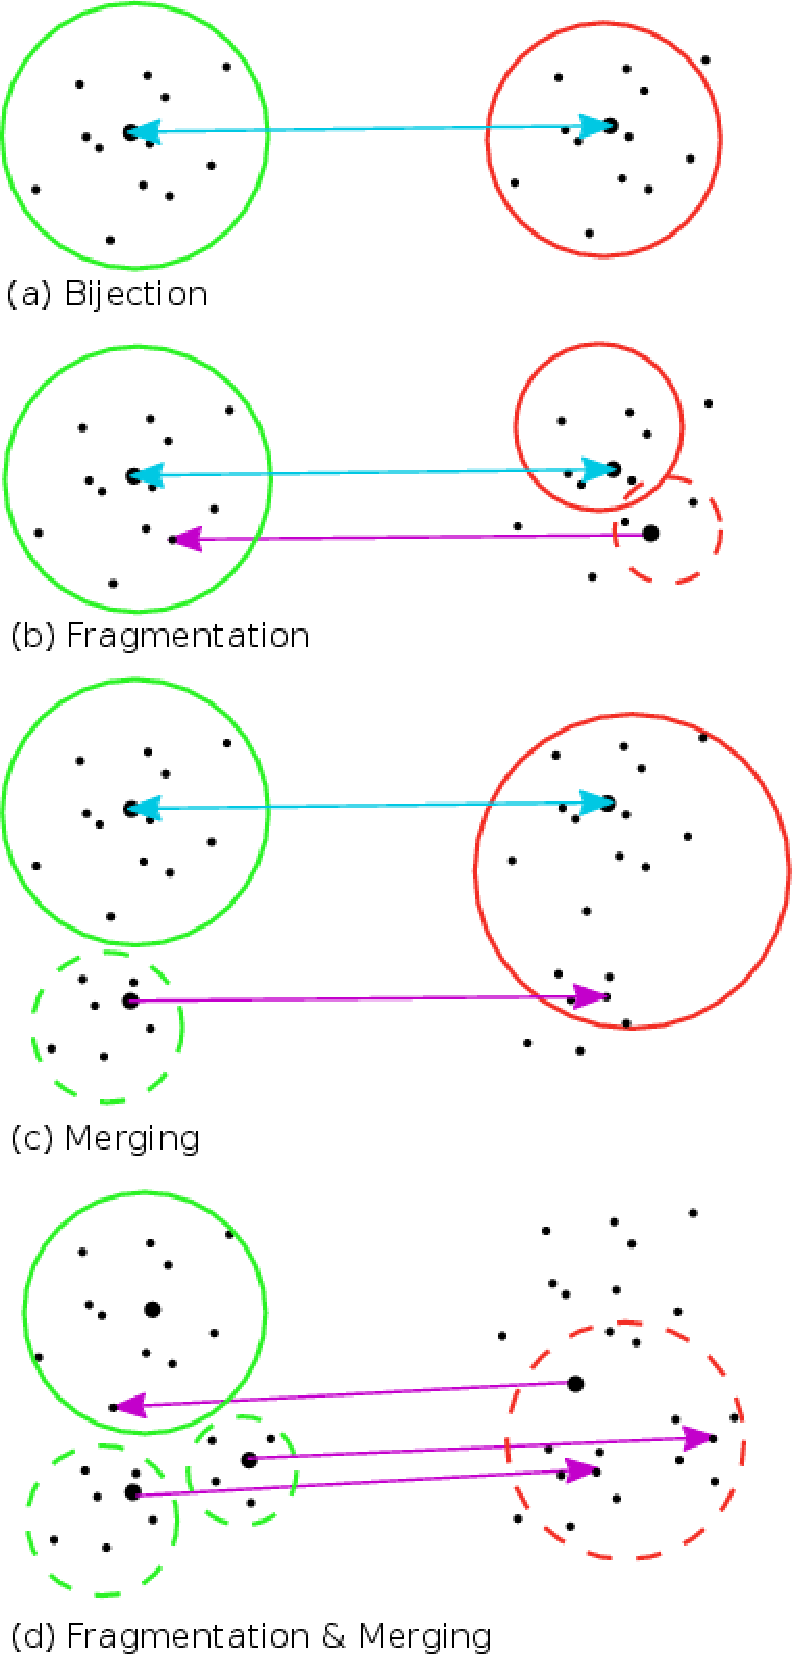
\includegraphics[width=0.3\linewidth]{figures/fof/bijection.pdf}%
    \caption{Schematic links between true groups (\emph{green circles}) and
    FoF-extracted groups, (\emph{red circles}), each with their respective
    most massive galaxy (\emph{black dots}).
    The \emph{solid circles } represent primary true and FoF groups, while the
    \emph{dashed circles} respectively correspond to secondary true groups and
    FoF fragments.
    The \emph{cyan double arrows} each indicate the one-to-one correspondence
    between the most massive galaxy in the true and extracted groups.
    The \emph{purple rightwards-pointing  arrows} correspond to the most
    massive galaxy of a true group ending up as a galaxy that is not the most
    massive of its extracted group.
    The \emph{purple leftwards-pointing arrows} represent the cases where the
    most massive galaxy of an extracted group is not the most massive of its
    parent true group.
\label{fig:CRdef}}
\end{figure}

\subsection{Global tests}

Our definition of the link between EGs and TGs allowed us to search for cases
where there is no one-to-one correspondence between the groups in real and
redshift space: a TG can suffer from  \emph{fragmentation} into several EGs,
while an EG can be built from the \emph{merging} of several TGs.

\bartreffigure{CRdef} illustrates different cases (following an analogous
figure in \citealp{Knobel+09}). The top panel shows a one-to-one correspondence
between the true and extracted groups.

We defined a fragmented TG as one that contains the MMGs of several EGs.
Multiple situations can cause fragmentation of TGs. In some cases, the FoF
algorithm fails to recover entire TGs, selecting instead its primary and
secondary substructures (see panel \bartreffigure{CRdef}b). In other cases, an
EG is mostly composed of galaxies from one TG, but the MMG of another TG is
`accidentally' linked  to the first TG\@. In consequence, the EG could be
linked to a TG providing only a single member galaxy to the EG, in comparison
with more members arising from another TG\@. When fragmentation occurred, we
distinguished the \emph{primary EG}, as that whose MMG corresponds to the MMG
of the parent TG, from the other EGs, which we called \emph{fragments}.

The dual of fragmentation is merging. In this situation, an EG contains the
MMGs of several TGs. Proceeding similarly as for the case of fragmentation, we
denoted \emph{primary TG} of a given EG the TG whose MMG corresponds to the MMG
of that EG, denoting the other TGs as \emph{secondary}. An example of merging
is shown in \bartreffigure{CRdef}c. Note that a true group can be fragmented
and its primary extracted group can be the result of a merger of the true group
with another one, as illustrated in \bartreffigure{CRdef}d.

\subsection{Local tests}
\label{sec:localtests}

Our local tests check the membership of the EGs. We defined \emph{completeness}
as the fraction of galaxies in the TG (i.e.\ within the sphere of radius
$r_{200}$) that were members of the primary EG\@. Given this definition, it did
not make sense to consider the completeness for secondary fragments, hence we
limited our tests to the primary EGs.

We defined \emph{reliability} as the fraction of galaxies in the EG that were
members of the parent TG (i.e., within the sphere of radius $r_{200}$). Here,
we also limited our tests to the primary EGs.

Mathematically speaking, these definitions of galaxy completeness, $C$, and
reliability, $R$, can respectively be written as
%
\begin{eqnarray}
    C=\rm \frac{TG \cap EG}{TG} \ ,\nonumber\\
    R=\rm \frac{TG \cap EG}{EG} \,. \nonumber
\end{eqnarray}

Looking at \bartreffigure{CRdef}, the completeness is the fraction of galaxies
in the TG (left, green circles) recovered in the EG (right, red circles), while
the reliability is the fraction of galaxies in the EG that belong to the TG\@.

These four quantities allow one to define the capacity of the FoF grouping
algorithm (or any other grouping algorithm) to recover groups in real space
from galaxy catalogs in redshift space.

Note that EGs that are fragments can have high reliability, while fragmentation
causes primary EGs to have reduced completeness. When EGs are mergers of TGs,
the secondary TGs lead to a decrease in the reliability, but can have high
completeness.

\subsection{Mass accuracy}

There are many properties of groups that one wishes to recover with optimal
accuracy (see Sect.~\ref{sec:fof_introduction}). We focused  here on one single
property that appeared to us as the most relevant: the group total mass. We
measured the masses of our EGs using the virial theorem formula of
\cite*{HTB85}
%
\begin{equation}
    M_{\rm EG} = {3\pi\over G}\,\langle R \rangle_{\rm h} \,\sigma_v^2
    = {3\pi\,N\over 2\,G}\,{\sum v_i^2\over \sum_{i<j} 1/R_{ij}}
    \ ,
\label{eq:MVT}
\end{equation}
%
where $\langle R \rangle_{\rm h} = \langle 1/R_{ij}\rangle^{-1}$ is the
harmonic mean projected separation, while $\sigma_v$ is the unbiased measure of
the standard deviation of the group velocities.

More precisely, we computed the accuracy of the log masses, respectively
defining the \emph{bias} and \emph{inefficiency} as the median and equivalent
standard deviation (half 16--84 interpercentile) of $\log (M_{\rm EG}/M_{\rm
TG})$, where $M_{\rm TG}$ is the mass of the TG within the sphere of radius
$r_{200}$ (see \bartrefsection{localtests}).

\subsection{Quality}

It is not simple to extract a unique pair of optimal LLs from the four tests
(fragmentation, merging, completeness, and reliability). To reduce the number
of tests, we combined fragmentation and merging into a single \emph{global
quality} and combined completeness and reliability into a single \emph{local
quality}.

We could define our qualities by multiplying $F$ (fragmentation) by $M$
(merging) and similarly, $C$ by $R$. However, one could alternatively multiply
$1-F$ by $1-M$, etc. Instead, we chose quality estimates that minimize the
distance to the perfect case. The advantage of using distance rather than
multiplying probabilities is that the former gives less weight to situations
where one of the two parameters is perfect and not the other. For example,
consider the case $F=M=p$. With the multiplication method, we would find that
$Q=p^2$ is also reached with $F=\epsilon\ll 1$, yielding $M_{\rm
mult}=p^2/\epsilon$, which can be quite large (hence plenty of merging). On the
other hand, with the distance method, we would find that $Q=p\sqrt{2}$ is also
reached with $F=\epsilon\ll1$ for $M_{\rm dist}\simeq p\sqrt{2}$, which is much
more restrictive. In a perfect algorithm, fragmentation and merging don't
occur, hence $F=M=0$ they are null. We therefore chose to minimize the
\emph{global quality}, defined as
%
\begin{equation}
    Q_{\rm global} = \sqrt{F^2+M^2}
\end{equation}
%
Moreover, in a perfect grouping algorithm, the EGs are fully complete and
reliable, i.e. $\langle C\rangle=\langle R\rangle=1$, where the means are over
all the groups of a mass bin. We, hereafter, drop the brackets, so that $C$ and
$R$ should now be understood as means over groups within mass bins. We then
define the \emph{local quality} as
%
\begin{equation}
    Q_{\mathrm{local}}=\sqrt{{\left(1-
    C\right)}^2+{\left(1- R\right)}^2} \,.
\end{equation}

Both global and local qualities tend to zero for a perfect galaxy group
algorithm. So the optimal LLs will be those that minimize $Q_{\rm global}$,
$Q_{\rm local}$, mass bias and mass inefficiency. The maximum possible value of
both qualities is $\sqrt{2}$.

\subsection{Scope of the tests}

We limit our tests to TGs containing at least 3 galaxies and that are not split
by the transformations of the simulation box (see \bartrefchapter{mock}).
Moreover, we only consider EGs with at least 3 galaxies and that do not lie
near the survey edges (the virial radius, 2.3 Mpc, of a true group of log mass
15.2 in solar units, placed at $z=z_{\min}=0.01$, i.e.\ at an angle of more
than $3\fdg27$) or redshift limits ($1.8\,v_{200} \approx 2.7 \,\sigma_v$, of
the same mass group, corresponding to $3073 \, \rm km \, s^{-1}$). Typically
60\% (sample 2) to 25\% (sample 6) of the groups are flagged. Finally, the
tests of galaxy completeness and reliability, as well as mass bias and
inefficiency are restricted to primary EGs of TGs (not fragments).

\section{Results}
\label{sec:results}
%
\begin{figure}
    \begin{minipage}{\linewidth}
        \centering
        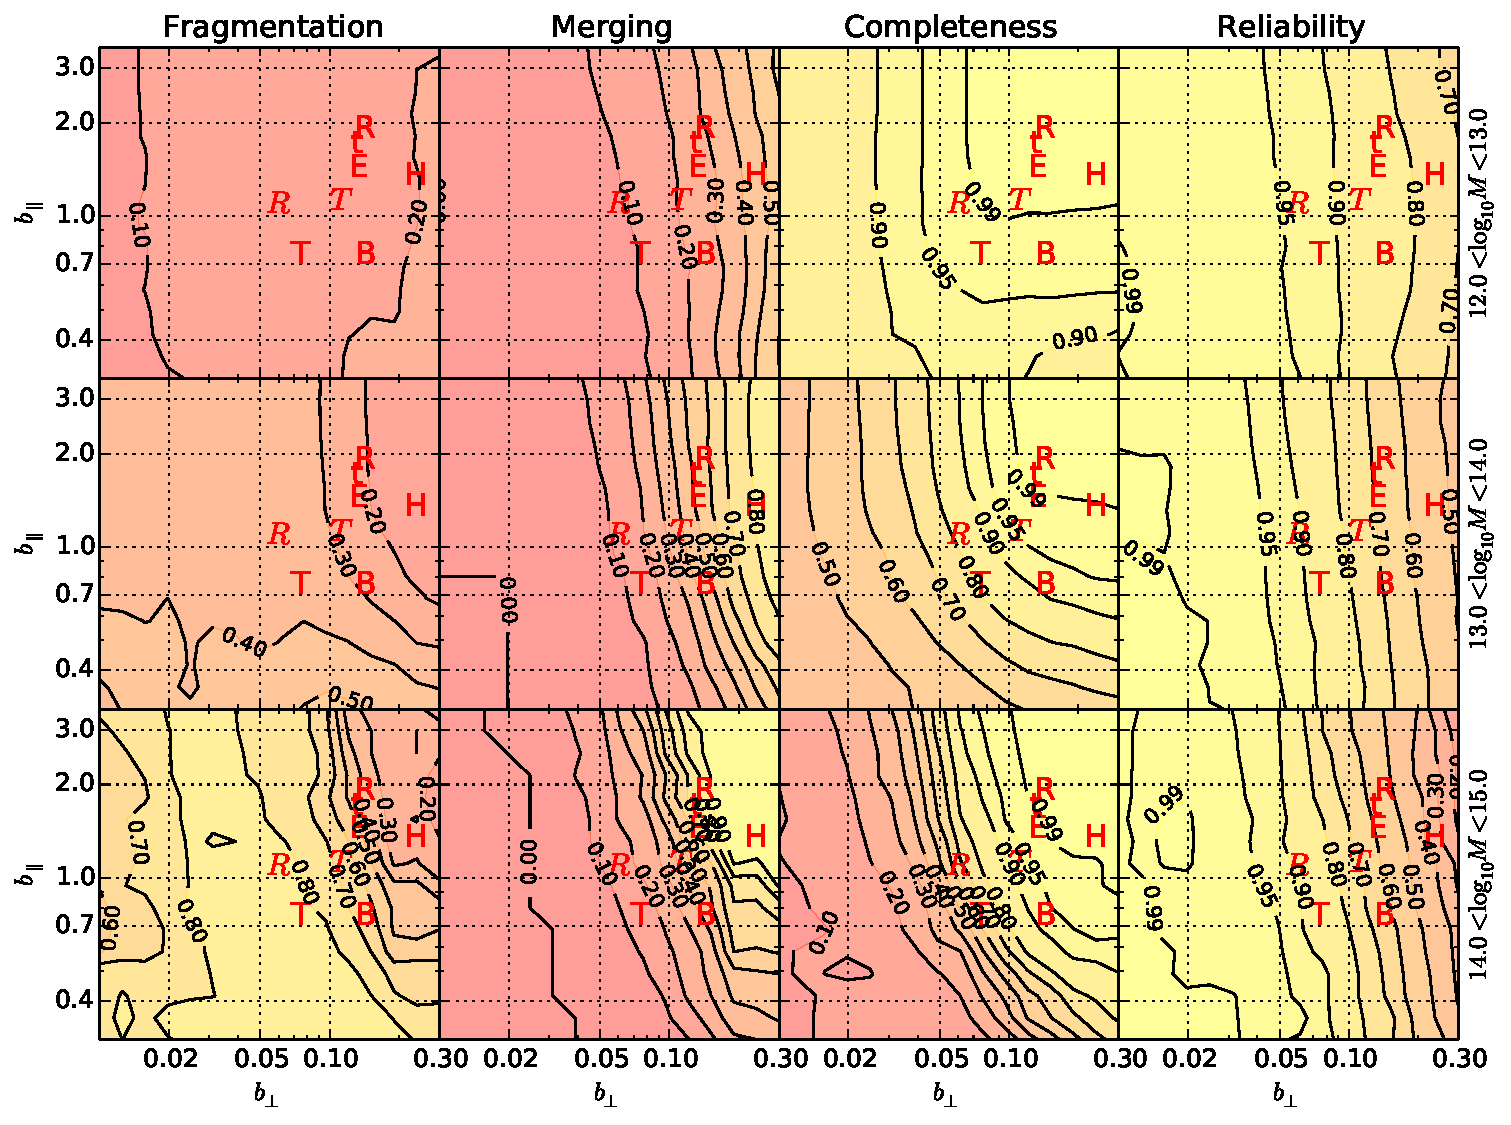
\includegraphics[height=0.415\textheight]{%
            figures/fof/results/mvir_true_1_fof_analysis.pdf%
        }
        \captionof{figure}{Contours of group fragmentation (\emph{first column}) and merging
            (\emph{second column}), as well as mean galaxy completeness
            (\emph{third column}) and reliability (\emph{fourth column}) computed
            for a 16$\times$16 grid of linking lengths for the nearby doubly
            complete galaxy subsample 2 in Table~\ref{tab:samples}. Results are
            shown for three bins of true group masses, for  unflagged groups of at
            least 3 members (for both the extracted and parent groups), and further
            restricted to primary groups in the completeness and reliability
            panels. Pairs of linking lengths corresponding to previous are also
            shown as \emph{red letters}
            (H\@: Huchra \& Geller 1982;
            R\@: Ramella et al. 1989;
            t:        Trasarti-Battistoni 1998;
            E\@: Eke et al. 2004;
            B\@: Berlind et al. 2006;
            T\@: Tago et al. 2010;
            $R$: Robotham et al. 2011;
        $T$: Tempel et al. 2014).\label{fig:test_true_small}}
    \end{minipage}
    \begin{minipage}{\linewidth}
        \centering
        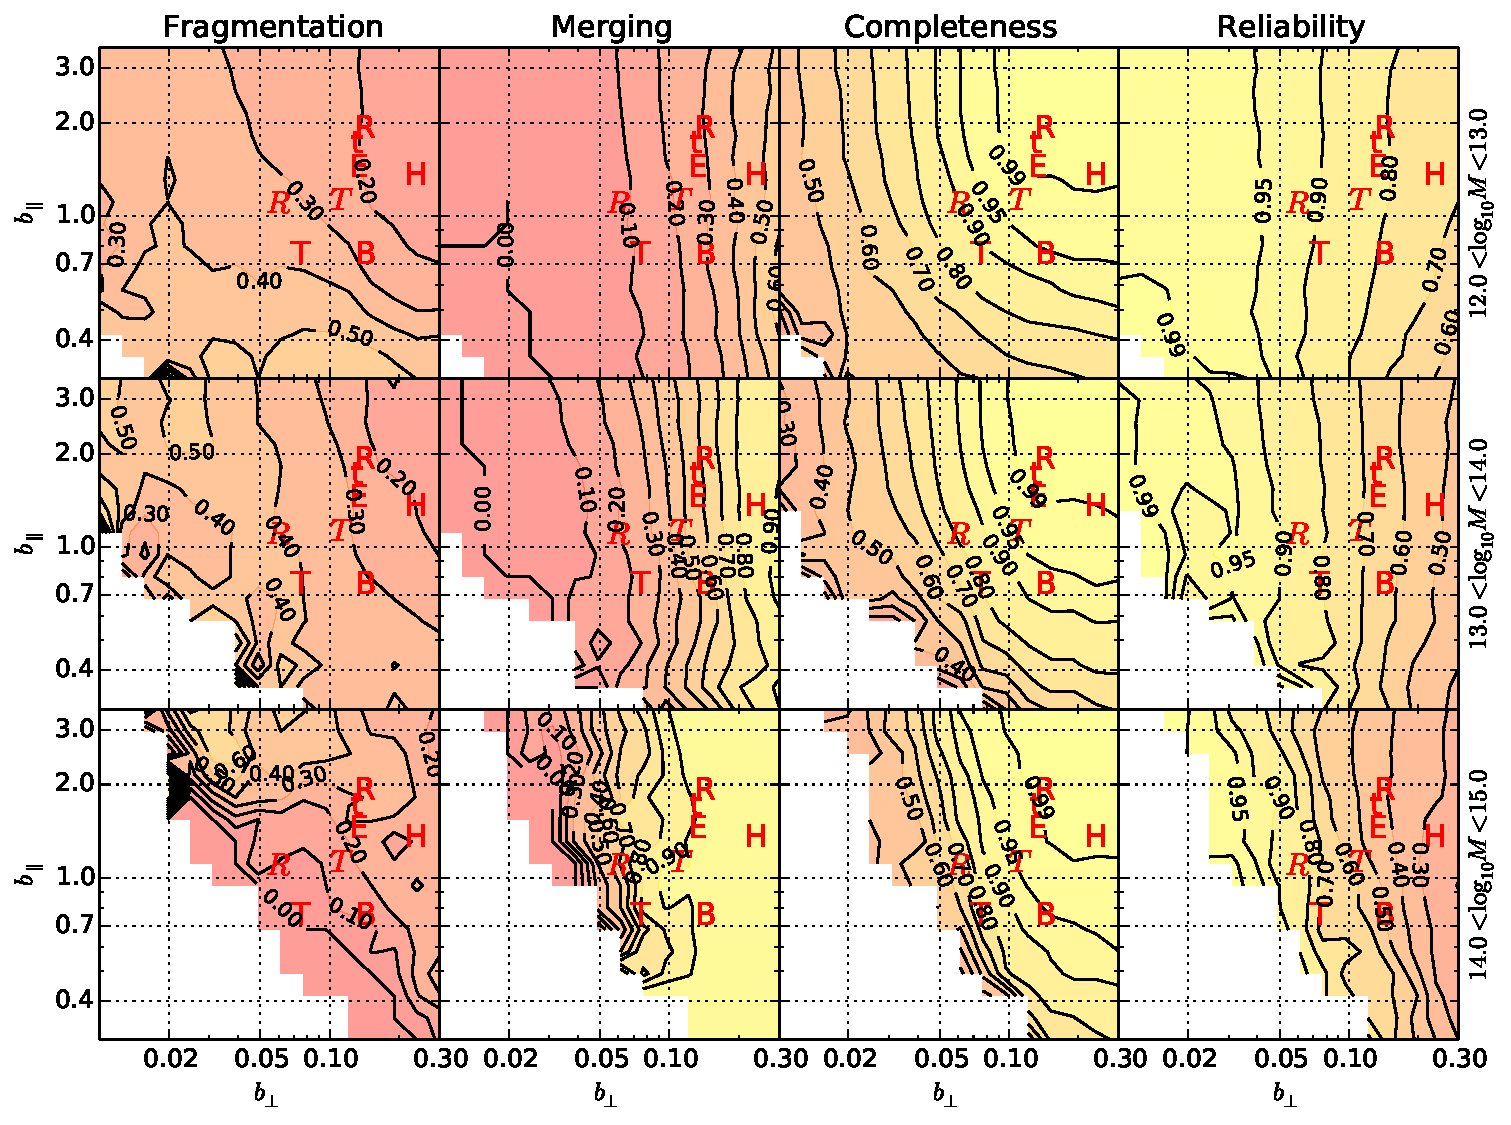
\includegraphics[height=0.415\textheight]{%
            figures/fof/results/halo_mass_1_fof_analysis.pdf%
        }
        \captionof{figure}{Same as \bartreffigure{test_true_small}, but where
        the different rows correspond to different bins of extracted group
    masses estimated from the virial theorem. The white zones show cases where
the linking lengths led to no unflagged groups extracted.
\label{fig:test_estimated_small}}
    \end{minipage}
\end{figure}
%
\begin{figure}
    \begin{minipage}{\linewidth}
        \centering
        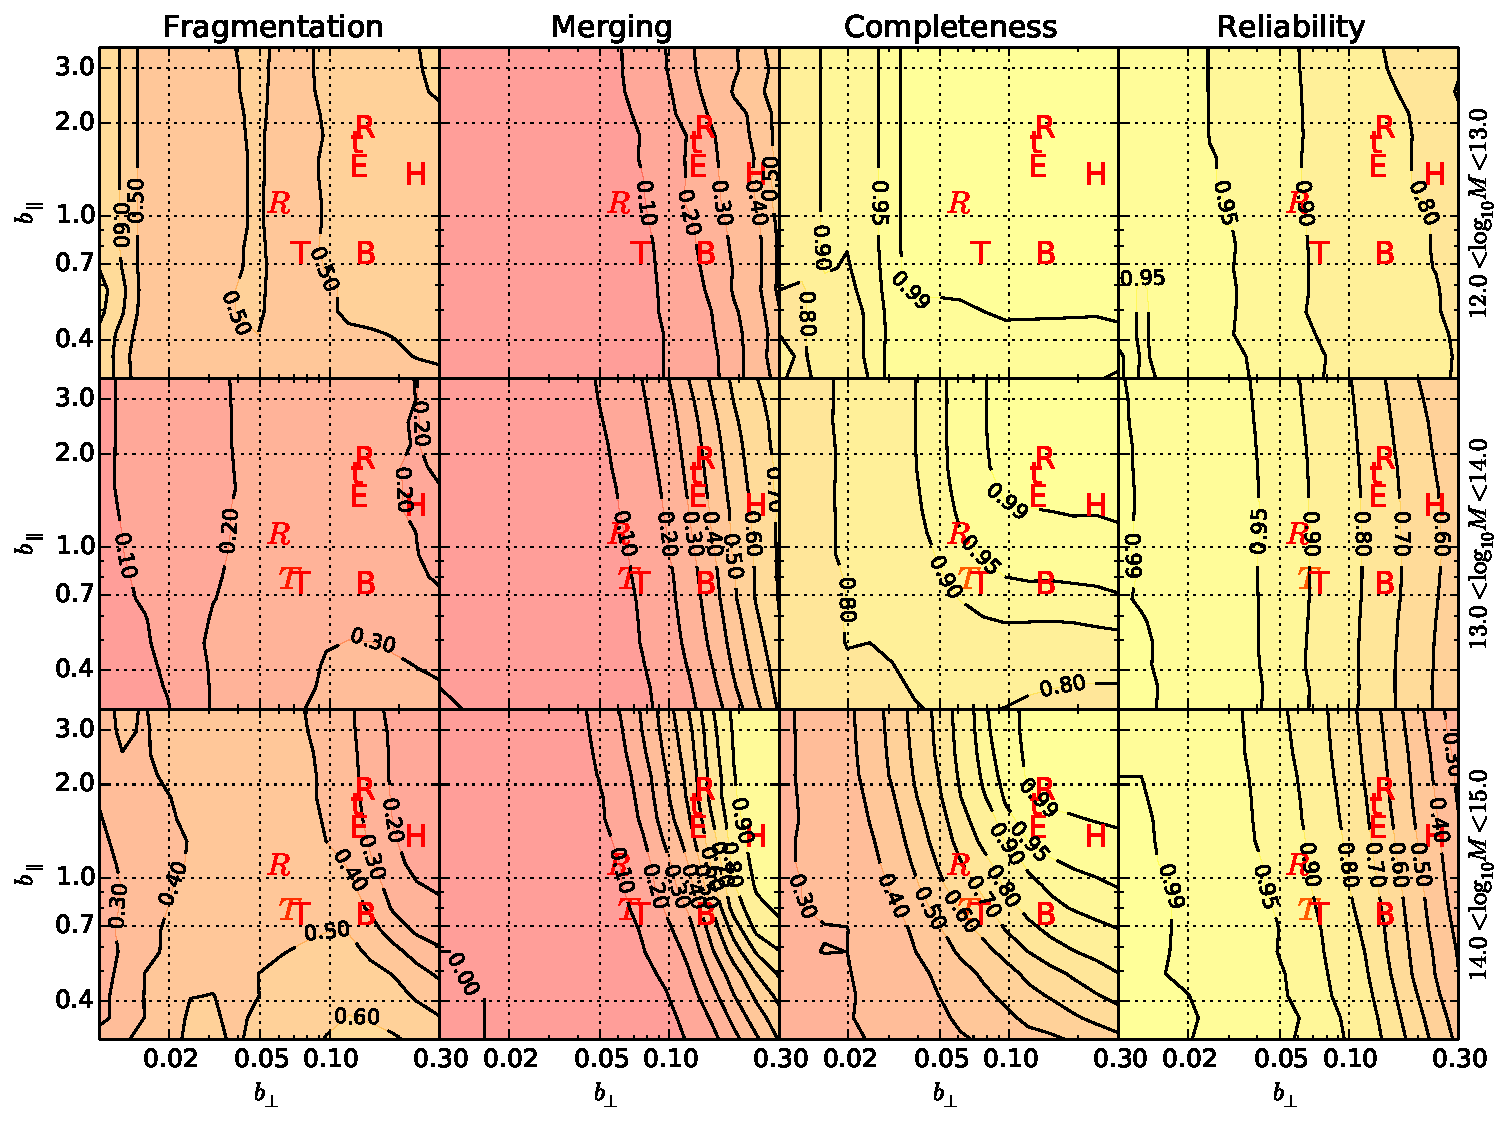
\includegraphics[height=0.415\textheight]{%
            figures/fof/results/mvir_true_5_fof_analysis.pdf%
        }
        \captionof{figure}{Same as \bartreffigure{test_true_small}, but for the
        distant doubly complete galaxy subsample 6 in
    Table~\ref{tab:samples}.\label{fig:test_true_big}}
    \end{minipage}
    \begin{minipage}{\linewidth}
        \centering
        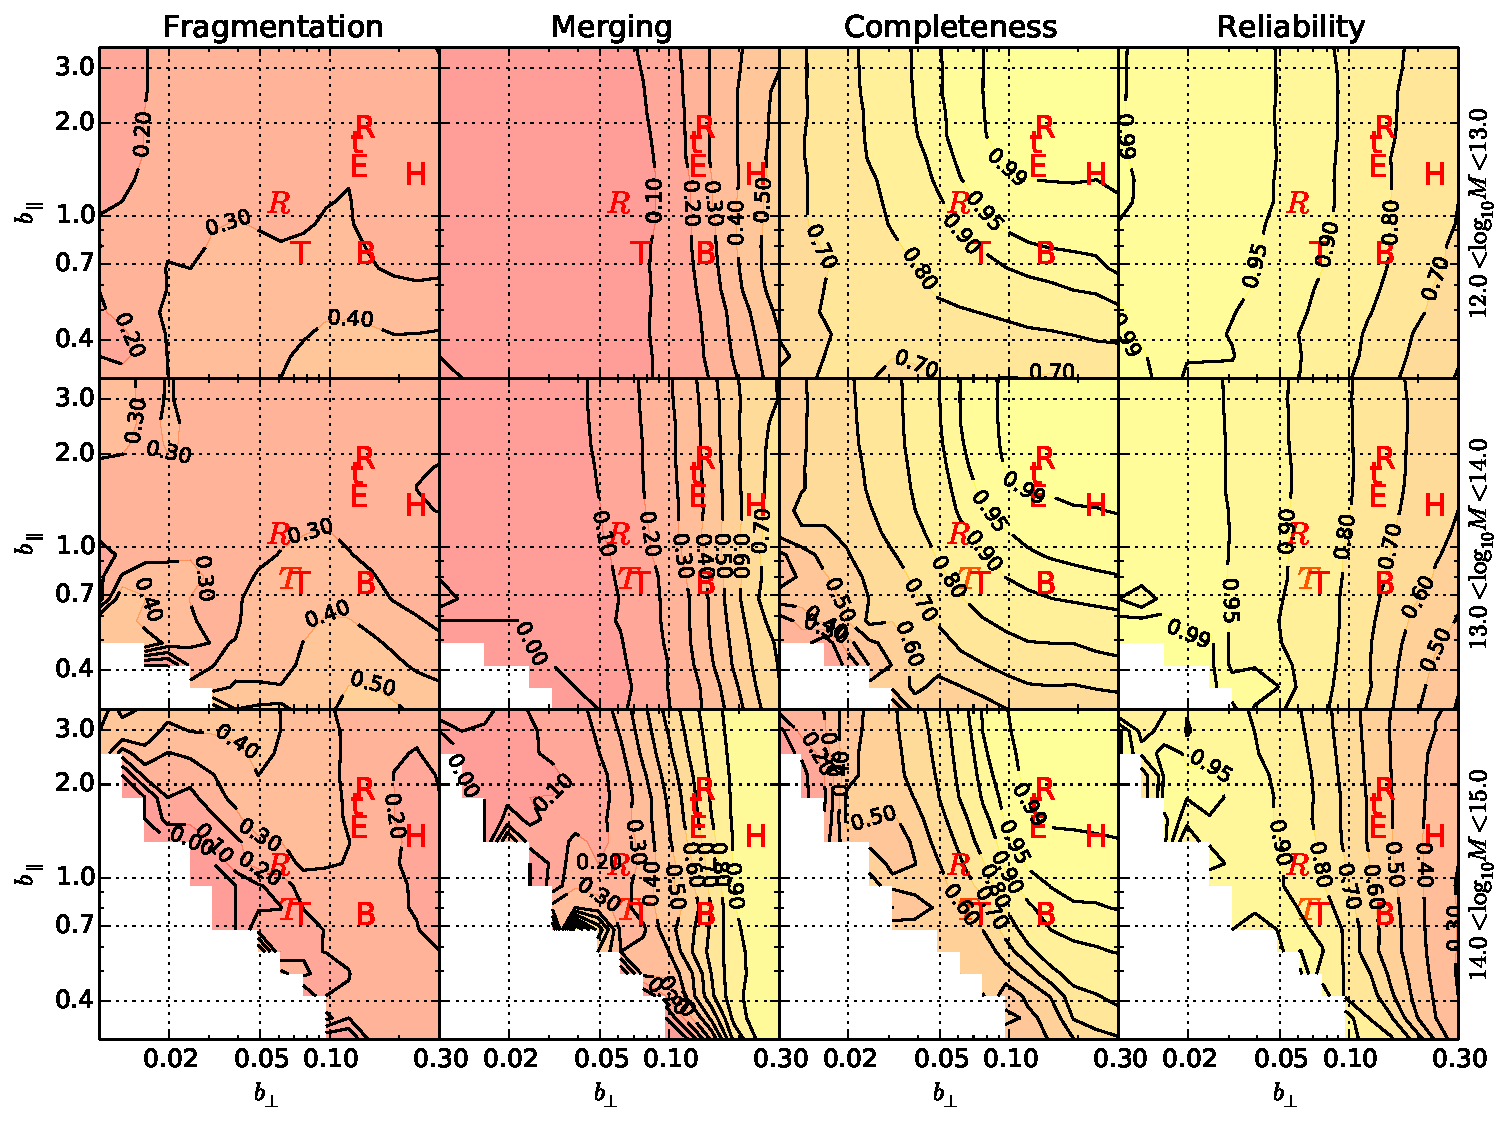
\includegraphics[height=0.415\textheight]{%
            figures/fof/results/halo_mass_5_fof_analysis.pdf%
        }
        \captionof{figure}{Same as \bartreffigure{test_true_big}, but where the
        different rows correspond to different bins of estimated
    masses.\label{fig:test_estimated_big}}
    \end{minipage}
\end{figure}
%
We have applied the FoF algorithm on near and distant doubly complete
subsamples (numbers 2 and 6 in Table~\ref{tab:samples}), repeating the tests
for a grid of 16$\times$16 geometrically-spaced pairs of LLs. The results of
our tests are shown in \bartreffigure{test_true_small} and
\bartreffigure{masses_diff}. The LLs of the different grouping studies listed
in Table~\ref{tab:groupalgos} are shown, except for~\cite{MZ02}, whose LLs
nearly overlap with those of~\cite{Eke+04}.

\subsection{Group fragmentation and merging}

\bartreffigure{test_true_small} indicates that, for the nearby doubly complete
subsample (number 2), fragmentation only affects the massive TGs (up to
$\approx$80\% of them for popular LLs), while
\bartreffigure{test_estimated_small} shows that, for popular LLs, the
fragmentation is lower (10--30\%) at high EG mass, hence fragment masses tend
to be small (typically 20--40\% fragmentation at small and intermediate
estimated masses).

On the other hand, the distant doubly complete subsample behaves in almost the
opposite manner: fragmentation is most important at the lowest TG masses
(roughly 50\% fragmentation, \bartreffigure{test_true_big}) and is independent
of estimated EG masses (at roughly 20--30\%,
\bartreffigure{test_estimated_big}).

In any event, fragmentation tends to decrease with greater linking lengths, as
expected, although it decreases somewhat faster with increasing $b_\perp$ than
with increasing $b_\parallel$.

Since merging is the dual of the fragmentation, one expects the level of
merging to vary  in the opposite way as fragmentation. Indeed,
\bartreffigure{test_estimated_small} and \bartreffigure{test_estimated_big}
indicate that merging becomes more important at higher estimated masses,
respectively reaching up to 90\% and 65\% for high estimated masses with
popular choices of LLs in subsamples numbers 2 and 6. However,
\bartreffigure{test_true_small} and \bartreffigure{test_true_big} shows that
the merging fraction increases only slowly with TG increasing mass, with
typically 15--40\% (increasing fast with $b_\perp$) of the TGs being merged with
other ones. Finally, merging decreases with smaller LLs, especially with
smaller $b_\perp$.
%
\begin{figure*}
    \centering
    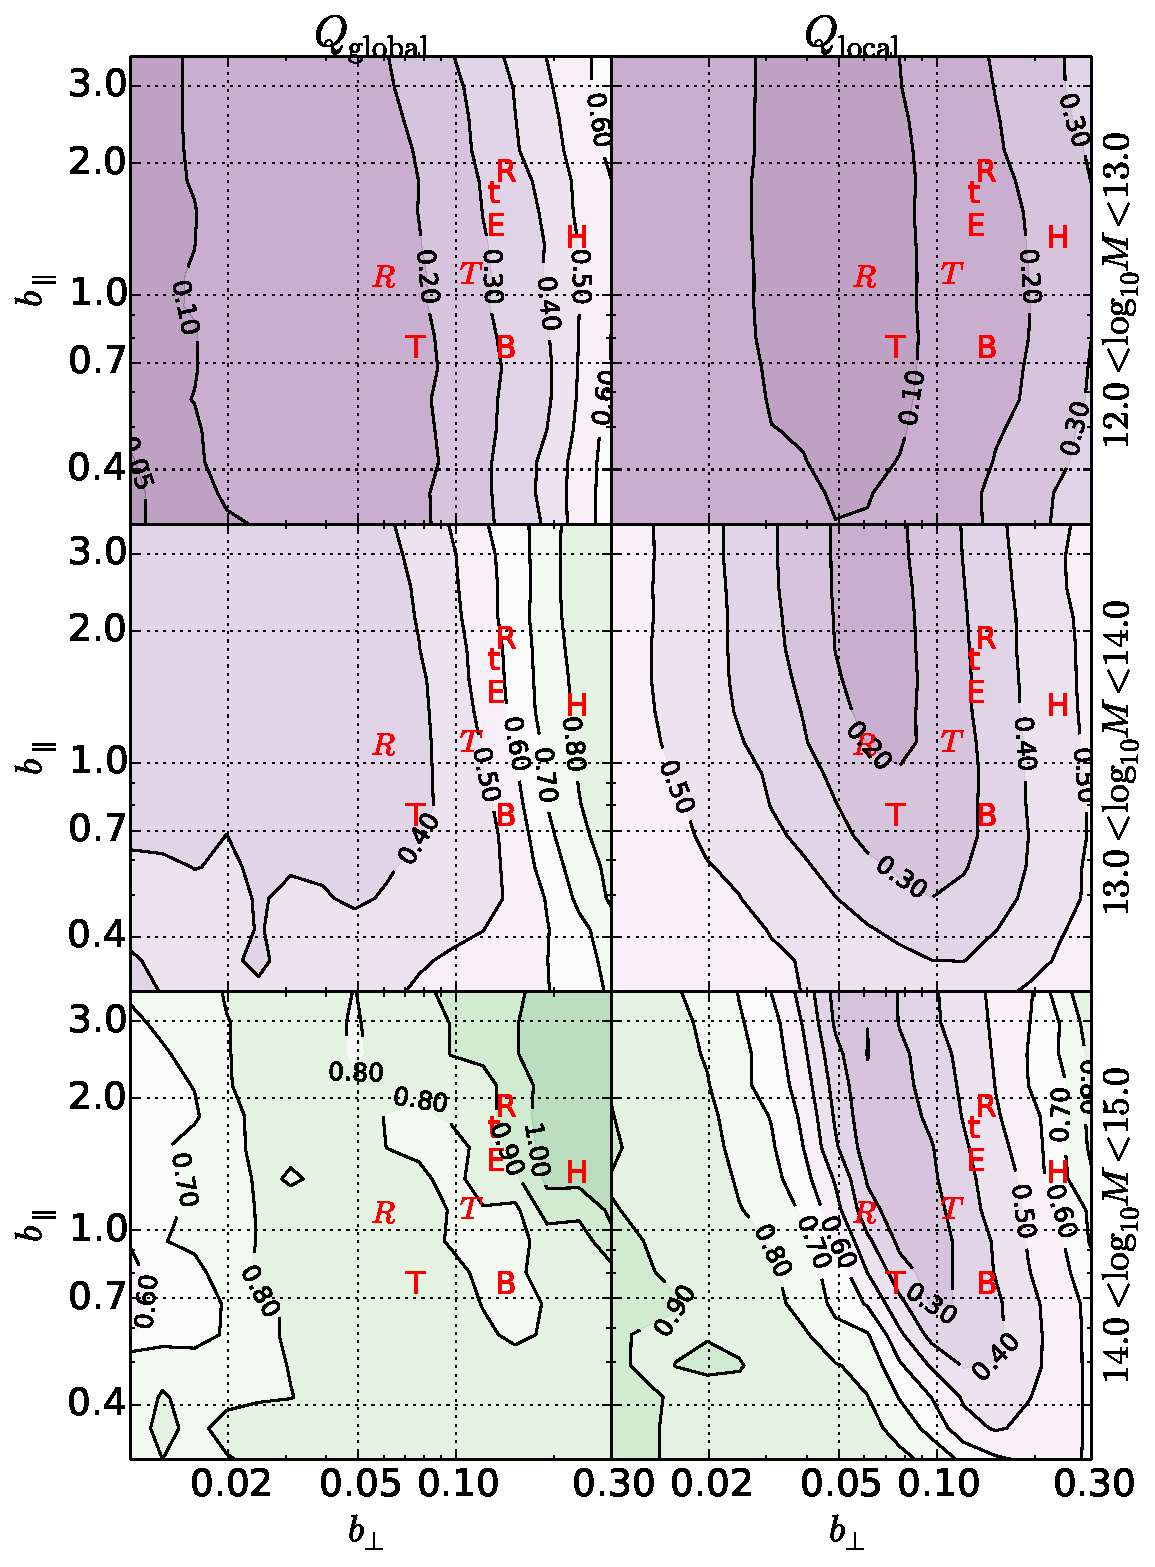
\includegraphics[height=0.4\textheight]{%
        figures/fof/results/mvir_true_1_quality_fof_analysis.pdf%
    }
    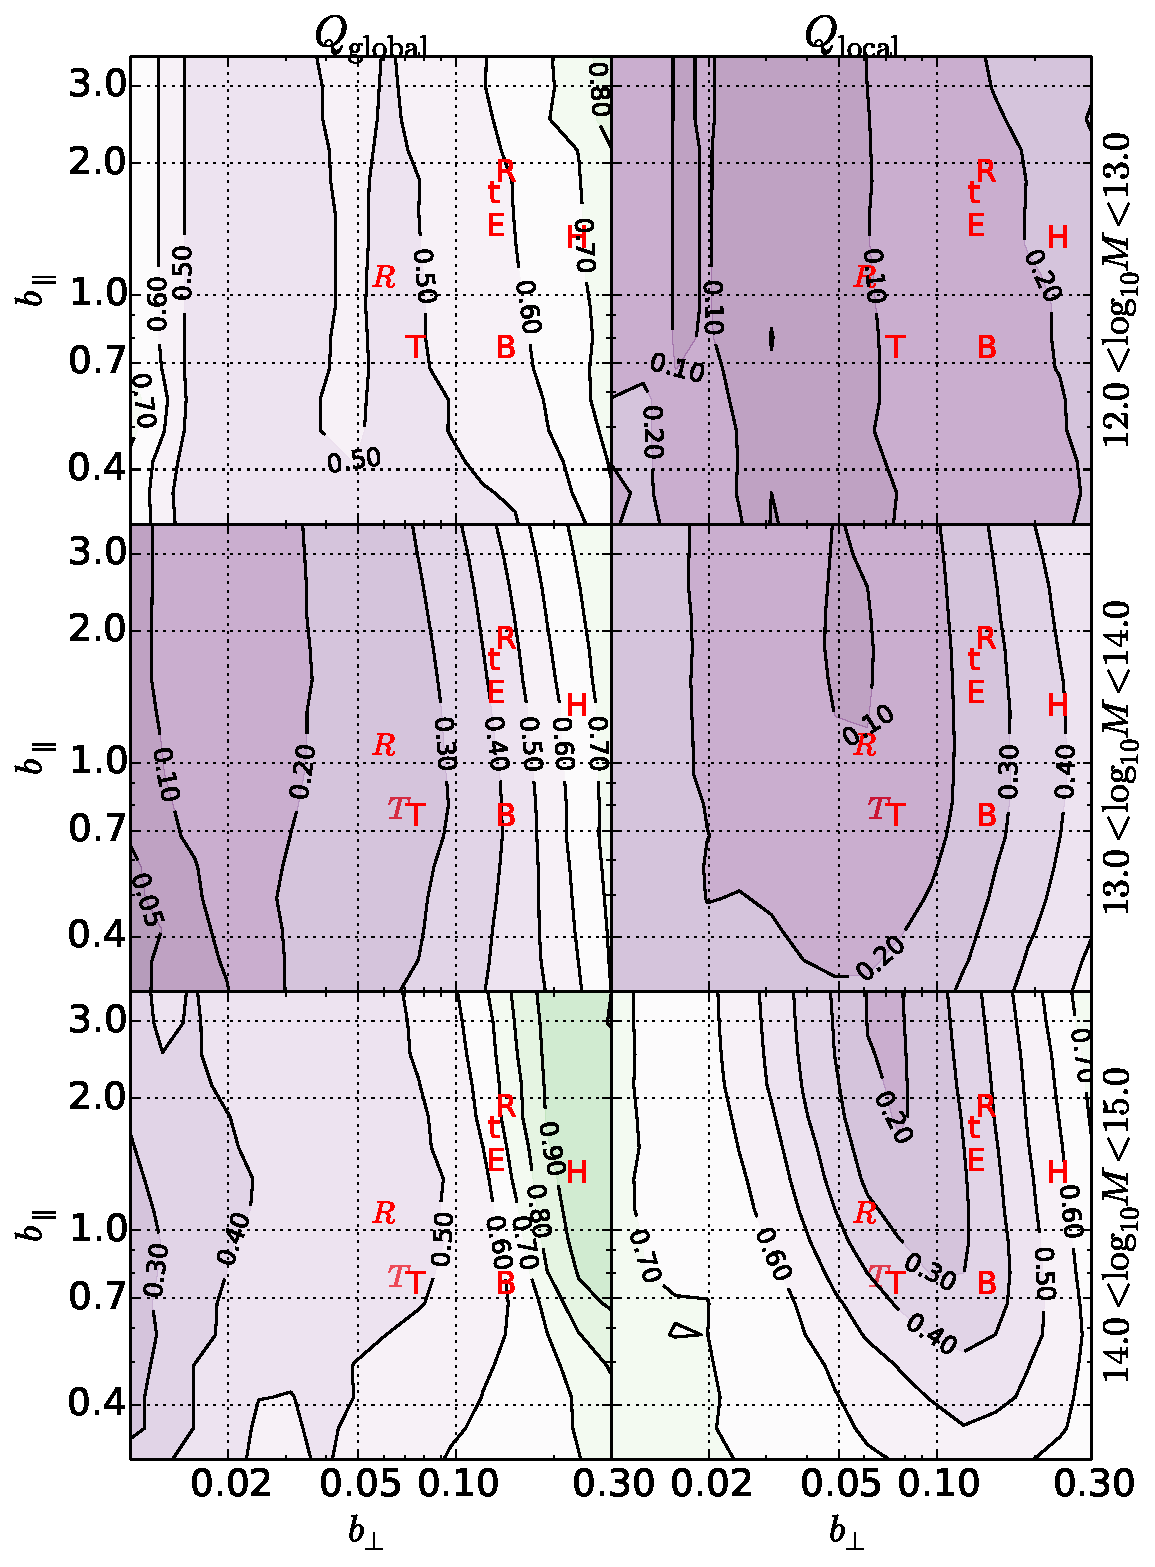
\includegraphics[height=0.4\textheight]{%
        figures/fof/results/mvir_true_5_quality_fof_analysis.pdf%
    }
    \caption{Global and local quality factors in a 16$\times$16 grid of linking
        lengths for subsamples 2 (\emph{left}) and 6 (\emph{right}), in three
        bins of true masses Results are shown for unflagged groups (restricted
        to primary groups for $Q_{\rm local}$) of at least 3 members (in both
    the true and extracted group). The symbols are as in
\bartreffigure{test_true_small}\label{fig:quality_true}}.
\end{figure*}
%
\begin{figure*}
    \centering
    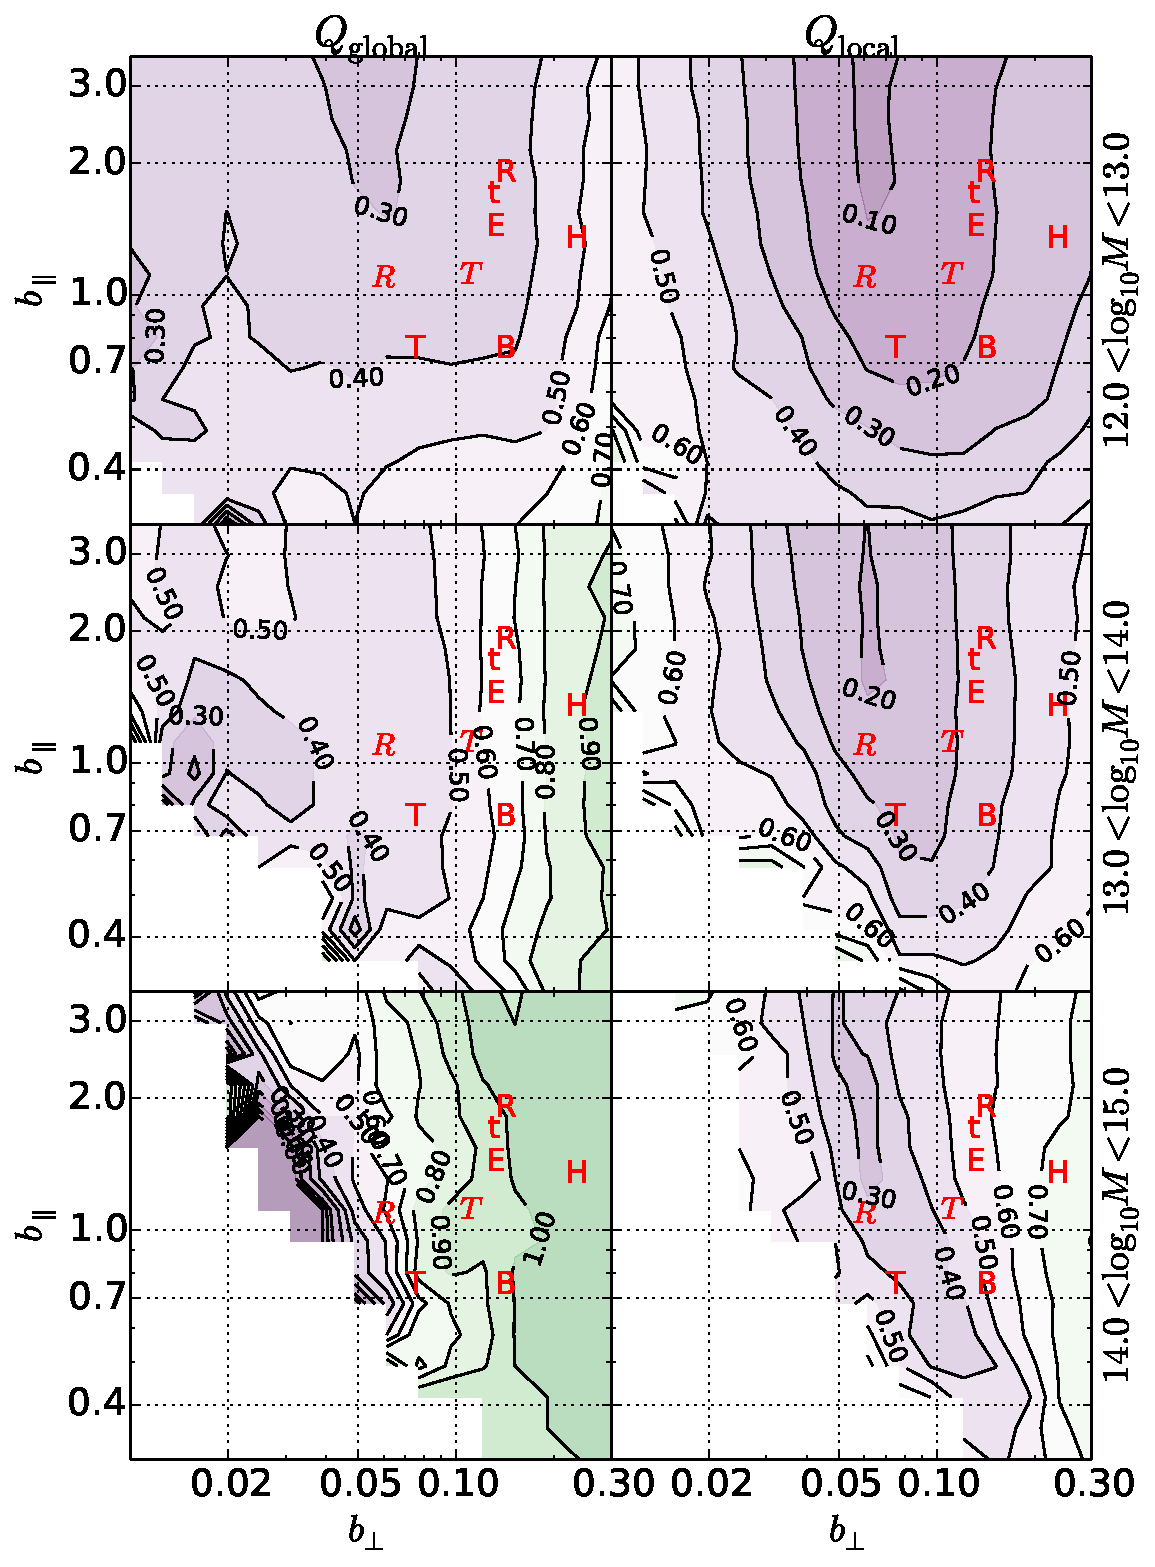
\includegraphics[height=0.4\textheight]{%
        figures/fof/results/halo_mass_1_quality_fof_analysis.pdf%
    }
    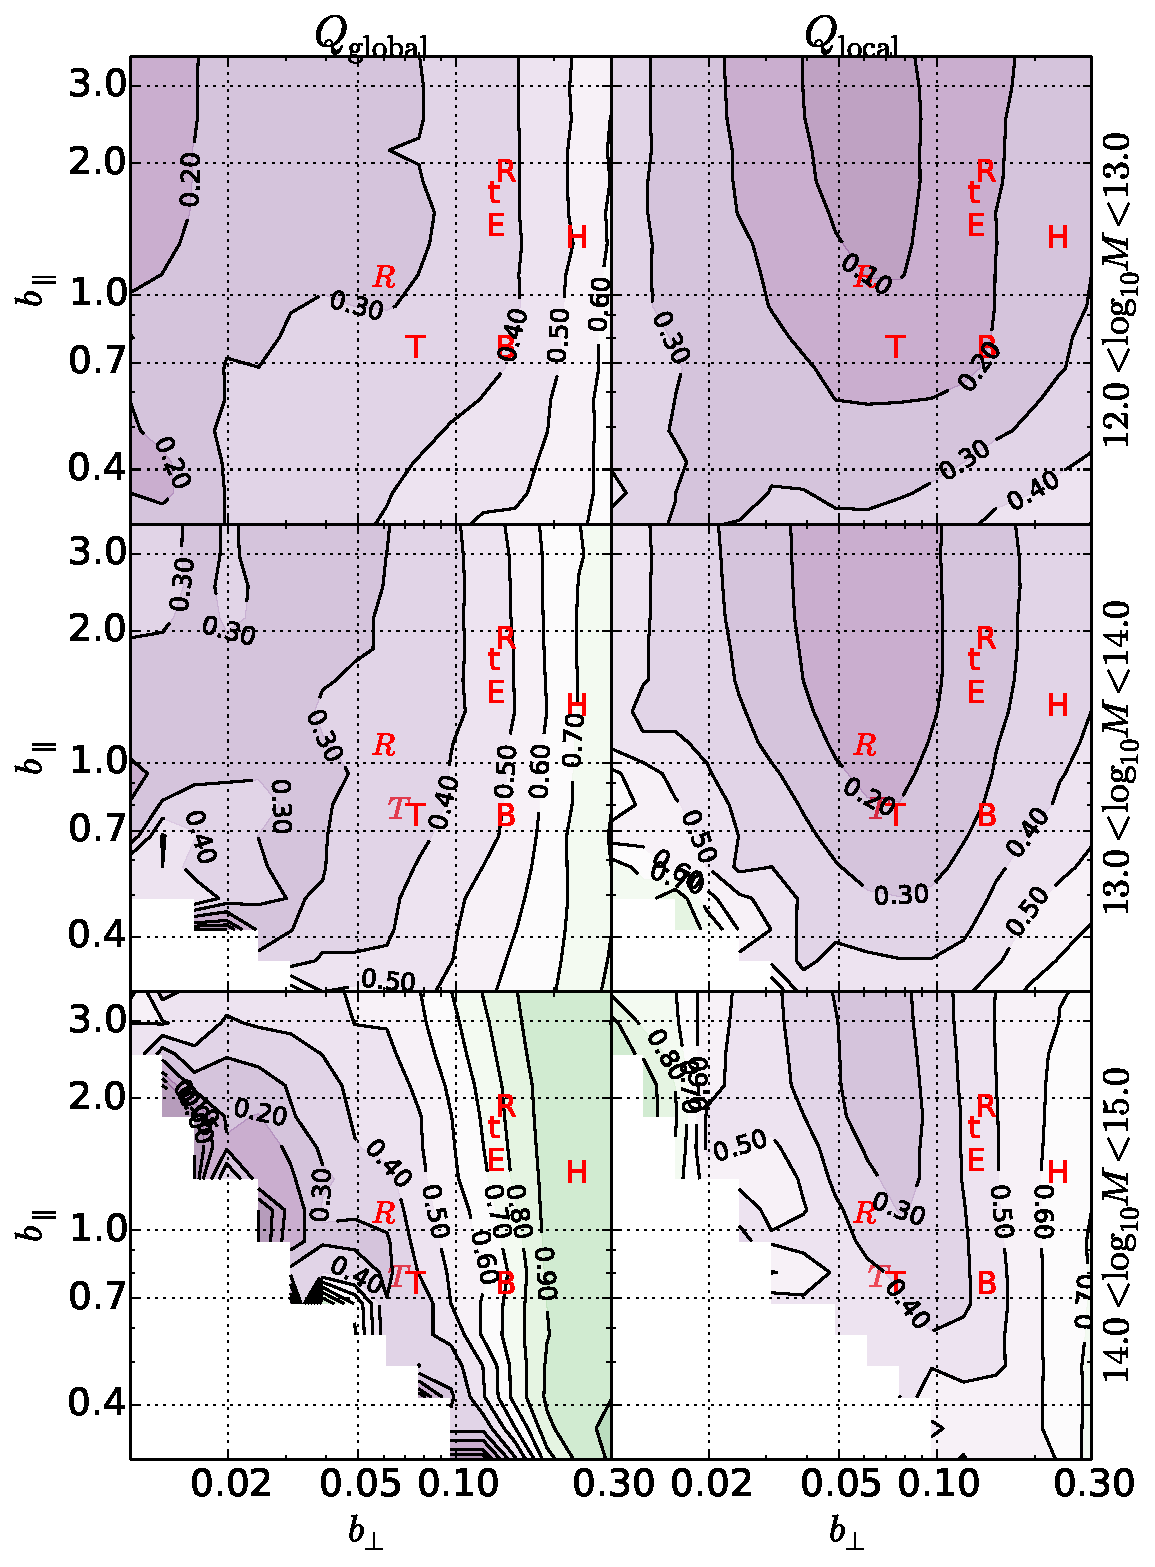
\includegraphics[height=0.4\textheight]{%
        figures/fof/results/halo_mass_5_quality_fof_analysis.pdf%
    }
    \caption{Same as \bartreffigure{quality_true} but in bins of estimated
    masses. The white zones show cases where the linking lengths led to no
unflagged groups extracted.\label{fig:quality_estimated}}
\end{figure*}

\bartreffigure{quality_true} and \bartreffigure{quality_estimated} show the
$Q_{\rm global}$ quality indicator that combines fragmentation and merging into
a single parameter. These figures show that decreasing $b_\perp$ leads to a
better tradeoff between fragmentation and merging, i.e.\ that the decrease of
merging with decreasing $b_\perp$ has a stronger effect than the increase of
fragmentation with decreasing $b_\perp$: the optimal $Q_{\rm global}$ is often
reached for $b_\perp < 0.02$.

\subsection{Galaxy completeness and reliability}

\bartreffigure{test_true_small} and \bartreffigure{test_true_big} indicate that
completeness is very high ($>99\%$) at low TG masses, and decreases to lower
values ($60-99\%$) at high TG mass. A weaker trend occurs when EG mass is
substituted for TG mass (see \bartreffigure{test_estimated_small} and
\bartreffigure{test_estimated_big}). Since high mass TGs are less complete,
their estimated masses should be smaller, and the EGs with high masses will be
the lucky complete ones, which explains the weaker trend of completeness with
EG mass. Note that we are only considering primary groups of at least 3
members. The transverse and LOS linking lengths have roughly the same impact on
galaxy completeness.

The reliability of the group membership decreases with increasing EG mass
(\bartreffigure{test_estimated_small} and \bartreffigure{test_estimated_big}):
regardless of the subsample, the reliability is 80--90\% for low mass EGs, but
only 50--85\% for high mass EGs. The value of $b_\parallel$ has virtually no
effect on galaxy reliability. We will discuss this lack of convergence of the
reliability with $b_\parallel$ in \bartrefsection{discussion}.

Galaxy reliability also decreases with the masses of the TGs, but the trend is
weaker (\bartreffigure{test_true_small} and \bartreffigure{test_true_big}): as
the reliability decreases from 85--95\% to 60--90\%, roughly independent of the
subsample.

The right panels of \bartreffigure{quality_true} and
\bartreffigure{quality_estimated} show that, again, the transverse LL appears
to be more decisive than the LOS one when combining galaxy completeness and
reliability into a single local quality factor.

\subsection{Mass accuracy}
%
\begin{figure}[t]
    \centering
    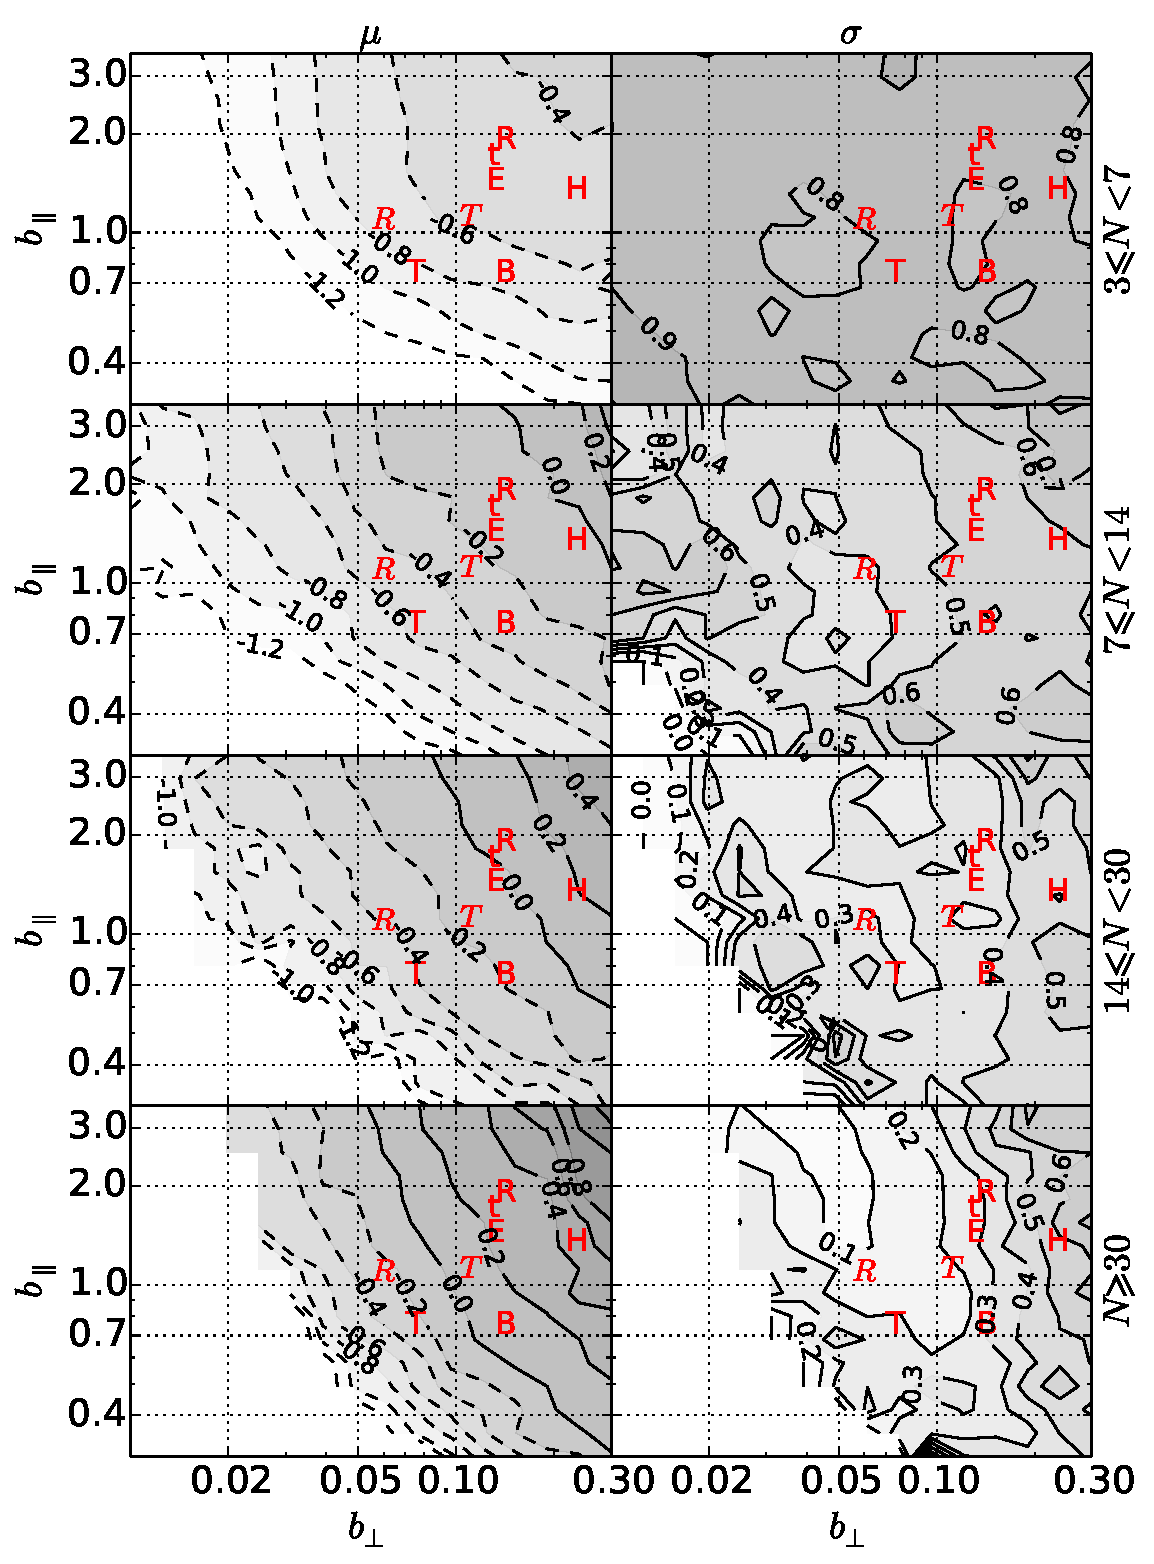
\includegraphics[height=0.44\textheight]{%
        figures/fof/results/1_fof_analysis_masses.pdf%
    }
    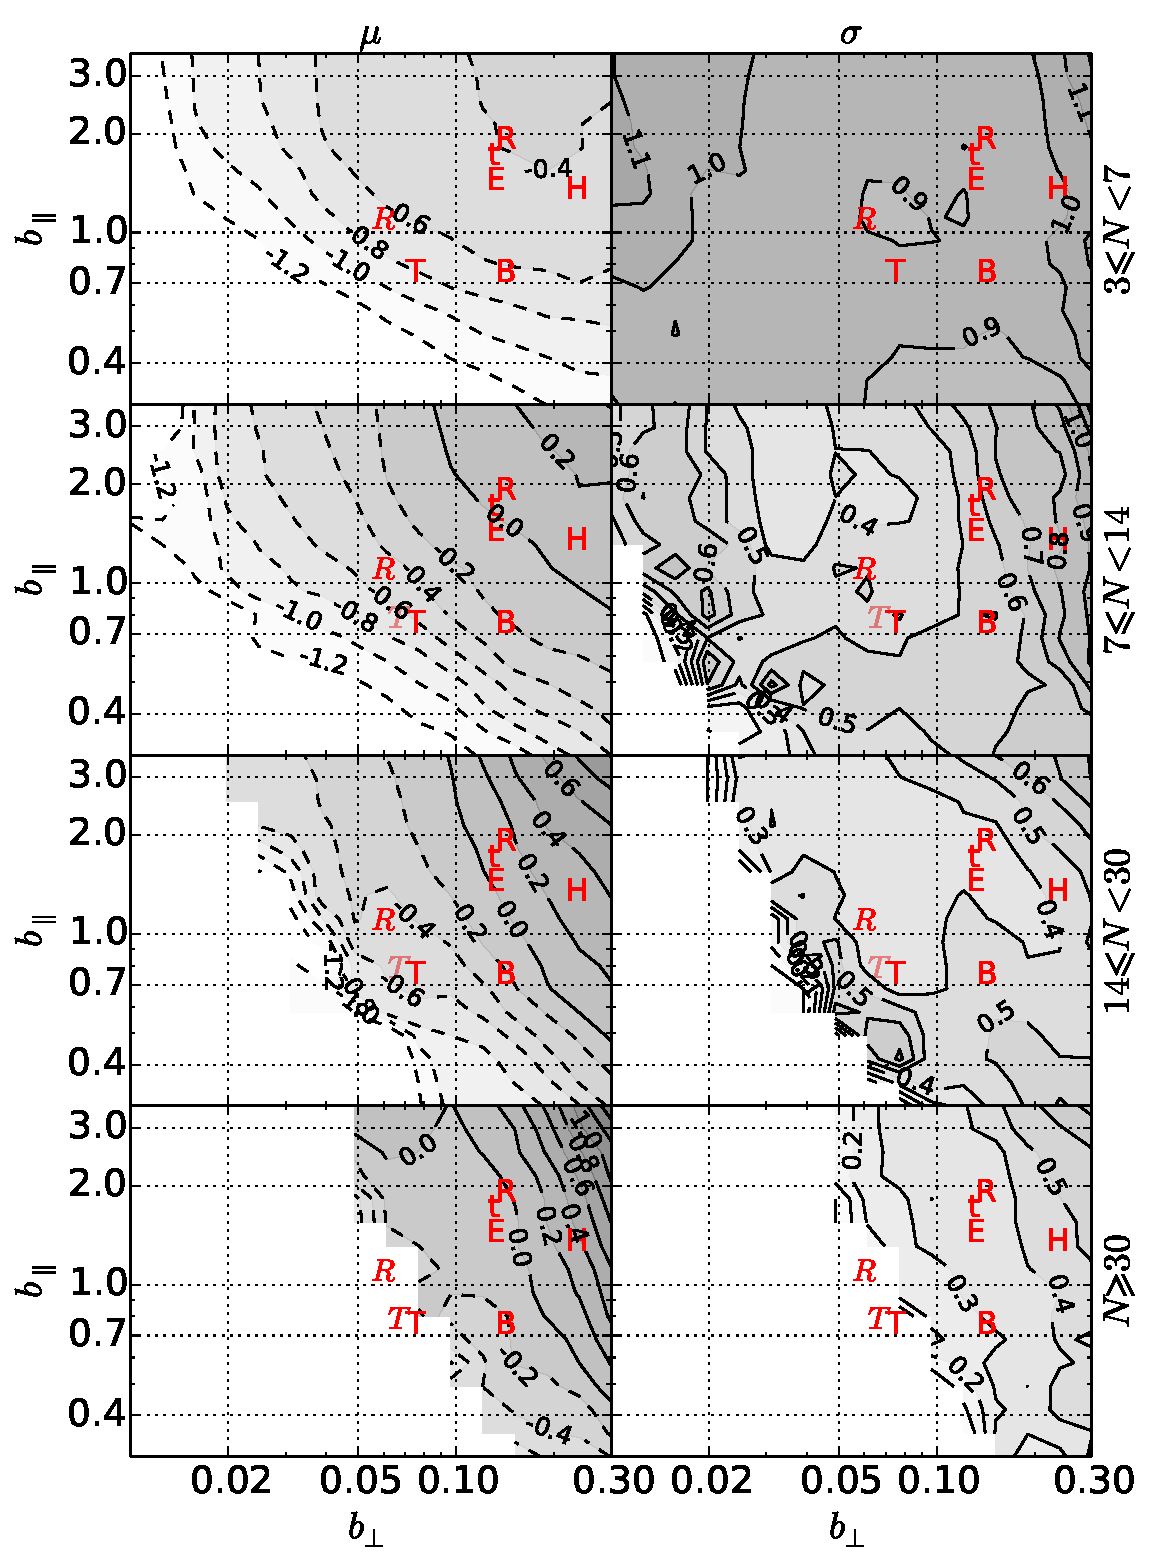
\includegraphics[height=0.44\textheight]{%
        figures/fof/results/5_fof_analysis_masses.pdf%
    }
    \caption{Bias ($\mu$) and inefficiency ($\sigma$) of the group masses
        estimated  by the virial theorem (\bartrefequation{MVT}) on our
        16$\times$16  grid of linking lengths, in four bins of extracted group
        richness (we do not consider extracted groups for which the parent true
        group has $\leq3$ members). The bias and inefficiency are respectively
        computed as the median and half 16--84 interpercentile of
        $\log_{10}\left(M_{\rm EG}/M_{\rm TG}\right)$. Results are shown for
        primary, unflagged groups. The left and right panels are respectively
        for galaxy subsamples 2 and 6. The symbols are as in
        \bartreffigure{test_true_small}. The white zones indicate linking
        lengths with no unflagged groups extracted.\label{fig:masses_diff}}
\end{figure}

The left columns  of the two panels of \bartreffigure{masses_diff} show that
the primary EG masses recovered by the FoF algorithm are systematically biased
low: for the popular choices of LLs, the bias ($\mu$) is as strong as
$-0.6\pm0.2$ dex at low multiplicity ($N_{\rm EG}\leq 6$), decreasing to
$0.0\pm0.3$ dex at high multiplicity ($N_{\rm EG}\geq 30$).

The right columns of the two panels of \bartreffigure{masses_diff} indicate
that, even if the biases could be corrected for, the masses cannot be recovered
to better than 0.8--0.9 dex at low multiplicity, improving to 0.2 dex at high
multiplicity. The  inefficiency ($\sigma$) is minimal for $b_\perp \approx
0.05$ (within a factor 2) and $b_\parallel \approx 1.0$ (low richness) or
$b_\parallel \ga 1.0$ (intermediate and high richness). For transverse LLs
within 40\% of $b_\perp=0.1$, the inefficiency is not very insensitive to
$b_\parallel$.

The situation becomes even worse when fragments are included in the statistics.
In this work, we have separated the accuracy of the group masses with the
occurrence of group fragmentation. But observers cannot tell if a group is a
fragment or a primary EG\@.

\section{Conclusions and Discussion}
\label{sec:discussion}

Before testing the FoF algorithm using a mock galaxy catalog in redshift space,
we first argued on physical grounds (\bartrefsection{fofpred}) that the
normalized transverse linking length, ought to be $b_\perp \approx 0.10$
(slightly increasing with richness) to extract 95\% of the galaxies within the
virial radius of NFW true groups.  We also argued that, restricting the
galaxies along the line-of-sight to $\pm1.65\,\sigma_v$ (95\% of the galaxies)
for groups defined to be 200 times denser than the critical density of the
Universe, requires $b_\parallel/b_\perp \approx 11$, hence $b_\parallel \simeq
1.1$. These LLs are estimated from our mocks that are based upon the
Millennium-II simulation that had adopted $\Omega_{\rm m}=0.25$. Converting to
$\Omega_{\rm m}=0.3$ yields $b_\perp=0.11$ and $b_\parallel=1.3$. Finally,
estimating the contamination by interlopers, we predict between 80\% (NFW model
extended outwards) to 90\% (NFW model truncated to sphere plus random
interlopers) galaxy reliability.
%
\begin{figure}[t]
    \begin{minipage}{0.5\linewidth}
        \centering
        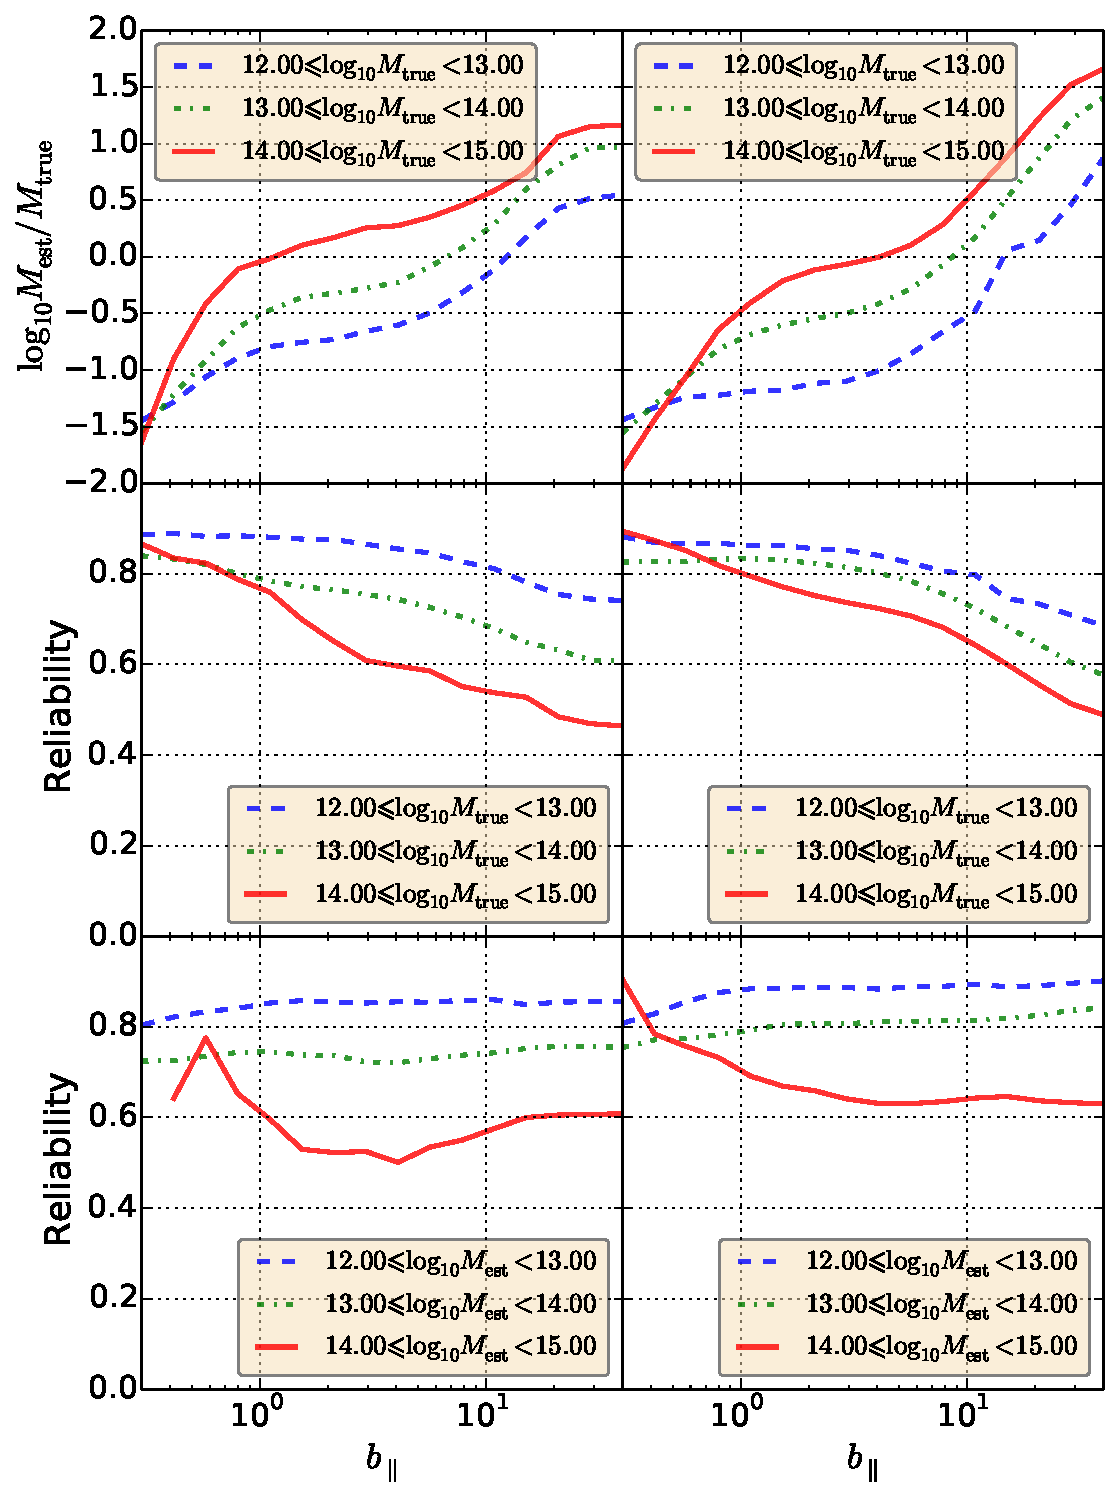
\includegraphics[width=0.85\linewidth]{%
            figures/fof/parallel_link_behaviour.pdf%
        }
        \captionof{figure}{Variation of the mass bias and reliability as a
        function of $b_\parallel$ for $b_\bot =0.1$, for subsamples 2
    (\emph{left}) and 6 (\emph{right}).\label{fig:parallel_behaviour}}
    \end{minipage}
    \begin{minipage}{0.5\linewidth}
        \centering
        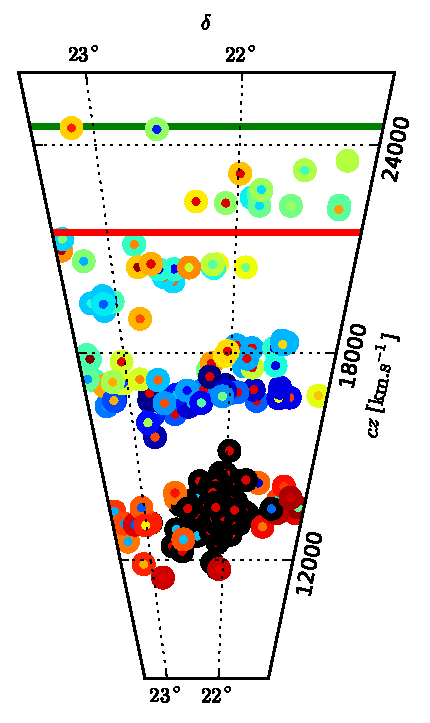
\includegraphics[width=0.6\linewidth]{figures/fof/group_halo.pdf}
        \captionof{figure}{An example of group and halo for $b_\parallel=20.8$
            and $b_\bot=0.1$ for subsample 4. The width of the cone is
            exaggerated by a factor of roughly 5 for illustrative purposes.
            \emph{Outer} and \emph{inner circle colors} respectively refer to
            the TGs and EGs. The \emph{horizontal green} and \emph{red lines}
            respectively indicate the maximum redshift, $z_{\max}$ and the
            redshift where galaxies are flagged for being close to $z_{\max}$.
            Some galaxies of the red EG, whose TG is the black one, are flagged
            for being close to $z_{\max}$, hence the group would not be
        considered in our tests.\label{fig:group}}
    \end{minipage}
\end{figure}

We then built a mock redshift space galaxy catalog with the properties of the
flux-limited SDSS primary spectroscopic sample, from which we extracted 2
subsamples that are doubly complete in distance and luminosity
(\bartrefchapter{mock}). We then extracted groups from both of these
subsamples, running the standard FoF algorithm for $16\times16$ pairs of
linking lengths.  In each case, we measured the fraction of true groups that
were fragmented in the FoF extraction process, the fraction of extracted groups
that were built by the merging of several true groups, as well as the bias and
inefficiency with which the group masses were extracted. Moreover, we computed
the completeness and reliability of the galaxy membership relative to the
spheres of radius $r_{200}$ in which the true groups are defined.

We analyzed group fragmentation, merging, galaxy completeness and reliability,
mass bias and inefficiency for two doubly complete subsamples and in bins of
true and estimated mass or estimated richness (for the mass accuracy).

We found that massive true groups are more prone to fragmentation, as expected,
but that, for popular choices of linking lengths, the probability of
fragmentation is greatest (30\%) at low estimated mass, i.e.\ the fragments are
of low mass. The process of fragmentation of rich (massive) groups  is similar
to images of large galaxies being preferentially fragmented by automatic image
extraction pipelines (e.g., \citealp{DePropris+07}).

Group merging is low at low estimated mass, but increases drastically to reach
40--90\% (for popular linking lengths) at high estimated mass. Galaxy
completeness is high, typically $>80\%$. Galaxy reliability is typically 75 to
90\% depending on group mass..

Our analytical prediction of 95\% completeness for $b_\perp\simeq 0.10$ is only
met for groups of high true masses (\bartreffigure{test_true_small} and
\bartreffigure{test_true_big}). Groups of low mass will have more concentrated
galaxy populations, which will lead to smaller values of ${\rm
Max}(S_\perp)/r_{200}$, hence smaller values of $b_\perp$. Also, our analytical
prediction of 80--90\% reliability for groups with $b_\perp=0.10,
b_\parallel=1.1$ is accurate for groups of all masses of the distant subsample
(\bartreffigure{test_true_big}). However, for the nearby subsample (2), our
predicted reliabilities are only \nobreak{accurate} for groups of low true
masses, but optimistic for higher mass groups, for which $R \simeq 70-75\%$.

Group merging and galaxy reliability depend little on $b_\parallel$, especially
at high transverse linking length, $b_\perp > 0.1$, where the galaxies are
extracted to projected radii beyond $r_{200}$, hence the contamination by
interlopers is mainly in the transverse direction. The lack of optimal
$b_\parallel$ for galaxy reliability may seem surprising at first. We checked
our analysis by measuring the reliability for $b_\perp=0.1$, for a very wide
range of $b_\parallel$ extending from 0.3 to 40.
%
The top panels of \bartreffigure{parallel_behaviour} indicate that the
reliability does end up decreasing fairly fast beyond some large value of
$b_\parallel \simeq 6$, i.e.\ beyond the limits of
\bartreffigure{test_true_small} and \bartreffigure{test_true_big}. The second
row of panels of \bartreffigure{parallel_behaviour} show a different behavior
in bins of estimated mass. This is the consequence of the estimated mass
increasing very fast with $b_\parallel$, as shown in the bottom panels of
\bartreffigure{parallel_behaviour}. The increase, with increasing
$b_\parallel$, of the mass bias is roughly parallel to the corresponding
decrease of the reliability (in bins of TG mass). At low $b_\parallel$, the
reliability decreases fairly rapidly and the mass bias increases rapidly
(towards zero), then both settle into an almost constant plateau in the range
$1.4 \la b_\parallel \la 8$, then both worsen rapidly up to $b_\parallel\simeq
25$, beyond which both saturate, because the longitudinal link is so large that
one reaches the minimum and maximum redshifts of the subsample, where most
groups are flagged. Massive groups that are built from TG merging can be fairly
reliable if the secondary TGs have negligible mass relative to the primary one.
This explains why $R$ remains fairly high when $M$ is high. The plateau around
\bpar$\approx 3$ appears to represent the range of optimal longitudinal LLs.

An illustration is given in \bartreffigure{group}, where a given EG has
reached the limits of the catalog with a very large value of \bpar{}.
\bartreffigure{group} also shows that interloping TGs are highly clustered.
This may explain why increasing $b_\parallel$ has only a small effect on
galaxy reliability: there is a void behind the main TG (black outer
circles).

While fragmentation, measured in bins of true group mass, decreases with
increasing $b_\parallel$, as expected (\bartreffigure{test_true_small} and
\bartreffigure{test_true_big}), we find that in bins of estimated mass, the
fraction of groups that are (secondary) fragments increases with $b_\parallel$
(\bartreffigure{test_estimated_small} and \bartreffigure{test_estimated_big}).
We believe that this is caused by interlopers increasing the group estimated
mass (\bartreffigure{parallel_behaviour}).

The masses, estimated with the virial theorem (\bartrefequation{MVT}) are a
strong function of the multiplicity of the extracted group. The estimated
masses are systematically biased low, especially for low extracted group
multiplicities (typically by a factor 4!). Similar trends have been found for
FoF groups \citep{Robotham+11} and for other, mostly dynamical, group mass
estimators \citep{Old+14}. The estimated group masses are inaccurate, even
after correcting for the biases: the typically errors are 0.8--0.9 dex at low
multiplicity, decreasing to 0.3 dex at high multiplicity.

The optimal completeness and reliability of the galaxy membership lead to
fairly extreme linking lengths, i.e. $b_\perp < 0.1$ and $b_\parallel > 2$.
However, the use of such a small transverse linking length amounts to
extracting the inner regions of groups, thus missing their outer envelopes.
Indeed, one notices that fragmentation worsens at increasingly lower values of
$b_\perp$. Therefore, our attempt to define a local quality by combining galaxy
completeness and reliability is of little use if one wishes to recover galaxies
out to close to the virial radii of groups.

In fact, the optimal linking lengths depend on the scientific goal:
%
\begin{itemize}
    \item statistical studies of environmental effects require high reliability
        (say $R>  0.9$), accurate masses and, to a lesser extent, minimal
        fragmentation.
    \item cosmographical studies of group mass functions require accurate
        masses, minimal group merging and fragmentation.
    \item studies for followups at non-optical wavelengths (e.g. X-rays),
        benefit from high completeness.
\end{itemize}

For statistical studies of environmental effects, it seems best to adopt
$b_\perp \simeq 0.06$, $b_\parallel \approx 1.0$, for which the reliability is
roughly as high as it gets for the choice of $b_\perp$: over 90\% at low
$M_{\rm EG}$ and over 80\% at intermediate and high $M_{\rm EG}$. Then,  the
completeness is higher than 70\% at high estimated mass and much higher at low
$M_{\rm EG}$. The mass inefficiency is minimal, but with this choice of LLs,
there will be virtually no EGs with more than 30 galaxies in the distant more
luminous subsample (\bartreffigure{masses_diff}).

This choice of LLs is close to that of~\cite{Robotham+11}, which may seem
obvious since both studies used some form of optimization of the LLs. However,
the details of the optimization criteria are somewhat different:
\citeauthor{Robotham+11} multiplied four criteria: basically the group
completeness and reliability, which bears some resemblance to our group
fragmentation and merging, but theirs is based on TG-EG pairs that have more
than half their galaxies in common, as well as two measures of a combination of
galaxy completeness and reliability, averaged over TGs and EGs respectively.
Our analysis differs in that we directly constrained group fragmentation and
merging, as well as galaxy completeness and reliability for primary fragments,
and finally mass accuracy.

For cosmographical and other studies involving accurate group mass functions,
it appears best to adopt $b_\perp \simeq 0.05$, $b_\parallel \simeq 2$, as
lower $b_\parallel$ increases fragmentation
(\bartreffigure{test_estimated_small} and \bartreffigure{test_estimated_big}),
while higher $b_\parallel$ causes too high group fragmentation at high EG
masses. This value of $b_\parallel\simeq 2$ is in agreement with the
intersection of the regions of $(b_\perp,b_\parallel)$ space  that optimize
both the multiplicity function  and velocity dispersions obtained by
\cite{Berlind+06}.

Finally, for non-optical followups, for which galaxy completeness is perhaps
the sole important parameter, one should privilege large linking lengths, e.g.
$b_\perp \simeq 0.2$, $b_\parallel \simeq 2-4$. However, one can also adopt
$b_\perp = 0.1$, $b_\parallel \simeq 2-4$, for which the completeness is
greater than 95\% at all masses and for both subsamples.

Converting from $\Omega_{\rm m} = 0.25$ (Millennium-II Simulation) to
$\Omega_{\rm m} = 0.3$ (WMAP-Planck compromise), $b_\perp$ must be increased by
6\% (\bartrefequation{bperpfromDelta}) to $b_\perp \simeq 0.07$ for the choices
optimizing environmental or cosmographical studies. Since $b_\parallel/b_\perp$
is independent of $\Omega_{\rm m}$ at given $\Delta$, \bpar{} must also be
increased by 6\%, i.e.\ to \bpar$\approx1.1$ for environmental studies.

We finally note that while high estimated mass group fragmentation  and merging
depends on the particular doubly complete subsample, galaxy completeness and
reliability as well as mass accuracy depend little on the
subsample.~\cite{Berlind+06} had similarly concluded that the doubly complete
subsample influenced little their tests of the group multiplicity function and
the accuracy of projected radii and velocity dispersions.

FoF grouping techniques can be used as a first guess for other more refined
grouping methods \citep{YMvdBJ05,Yang+07}. In a future paper \citep{DM14b}, we
will present another grouping algorithm, which is not an FoF, but is instead a
probabilistic grouping algorithm that is built upon our current knowledge of
groups and clusters (partly from X-rays and independent of FoF analyses of
optical galaxy samples) and from cosmological $N$ body simulations.

% vim: set tw=79 ft=tex:
